\part{Graph Traversals and Applications}
\label{ch:traversal}

\chapter{Graph traversal algorithms} %----------------------------------------
Traversals involve visiting each node of a digraph in a systematic way following only the arcs in the digraph. 
This is a very common task when dealing with digraphs and we will cover several applications in later lectures.

\section{The general graph traversal algorithm} \label{sec:trav}
All graph traversal algorithms have the same basic structure that relies on keeping track of which nodes have been visited 
and whether they may be adjacent to nodes that have not yet been visited. We use a system of three colours:
\begin{itemize} 
  \item \defnfont{White nodes} have not yet been visited;
  \item \defnfont{Grey nodes} (or \boldfont{frontier nodes}) have been visited but may have
  out-neighbours that are white;
  \item \defnfont{Black nodes} have been visited and all their out-neighbours have been visited too (so are not white). 
\end{itemize} 

\begin{Boxample}
Node states during a digraph traversal.
\begin{center}
  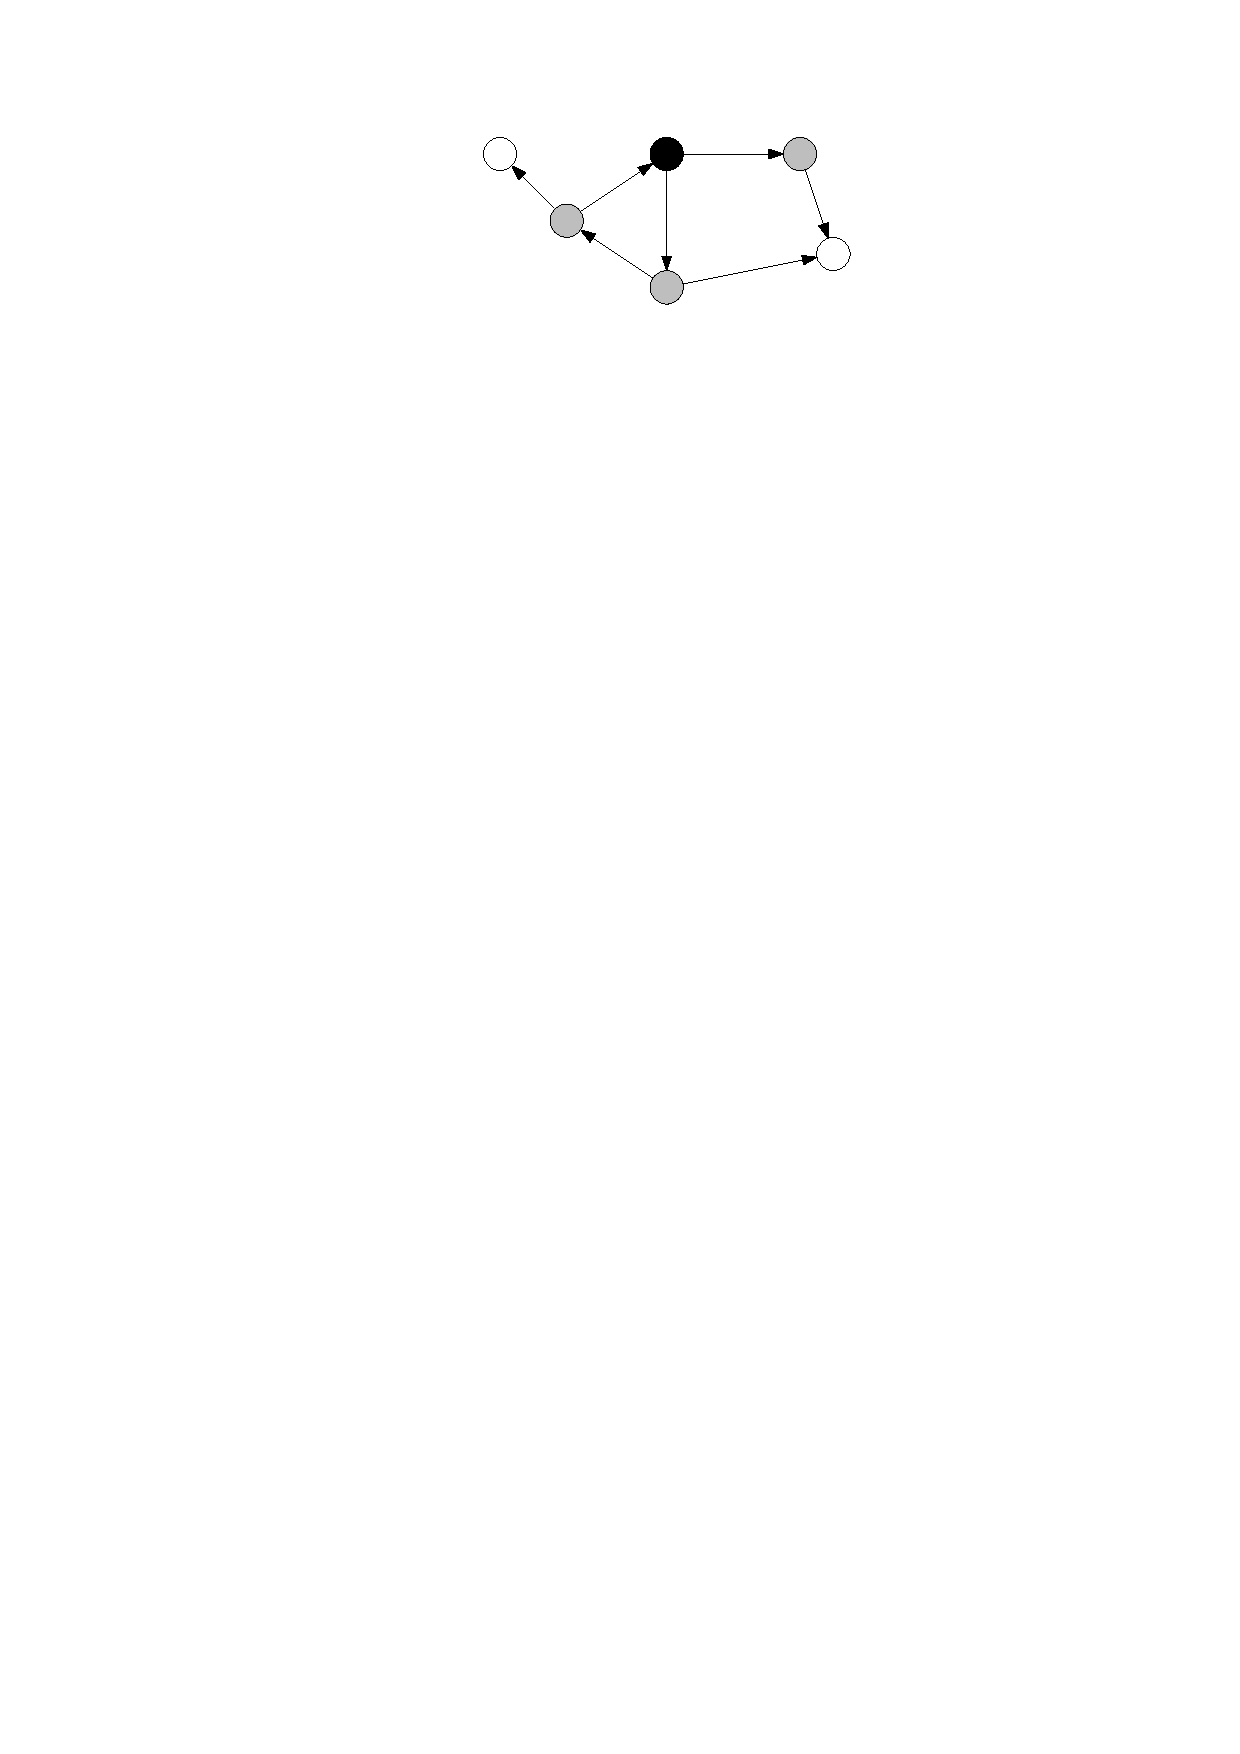
\includegraphics{graphTraversalNodeStateBW}
\end{center}
\end{Boxample}

The traversal algorithm which visits all nodes in a digraph is loosely described as follows: 
\begin{itemize}
  \item All nodes are white to begin with.
  \item A starting white node is chosen and turned grey.
  \item A grey node is chosen and its out-neighbours explored. 
  \item If any out-neighbour is white, it is visited and turned grey. 
  If no out-neighbours are white, the grey node is turned black. 
  \item The process of choosing grey nodes and exploring neighbours is continued 
  until all nodes reachable from the initial node are black.
  \item If any white nodes remain in the digraph, a new starting node is chosen 
  and the process continues until all nodes are black.
\end{itemize}

We keep track of the order in which nodes are visited by recording which arc was followed when a node first turned from white to grey. 
As we will see, this creates a sub-digraph of the original digraph which has a tree structure.

The traversal algorithm is formalised in the pseudocode of \cref{alg:traverse,alg:visit}.  
\cref{alg:traverse} (\algfont{traverse}) initialises the process and is tasked with finding white nodes to start from. 
Most of the work is done in \cref{alg:visit} (\algfont{visit}) which takes a starting node 
and explores the portion of the subgraph reachable from that node.

\begin{algorithm}[H]
  \caption{Basic graph traversal main routine: \algfont{traverse}}
  \label{alg:traverse}
\begin{algorithmic}[1]
\Function{traverse}{digraph $G$}
	\State array $\colour[0..n-1]$ \Comment{records node colour}
	\State array $\pred[0..n-1]$ \Comment{records path of traversal as a tree}
	\For{$u \in V(G)$} \Comment{make all nodes white}
		\State $\colour[u] \gets $ WHITE 
	\EndFor
	\For{$s \in V(G)$}  \Comment{find a white node}
		\If {$\colour[s] ==$ WHITE} 
			\State \texttt{visit}$(s)$ \Comment{start traversal from $s$}
		\EndIf
	\EndFor
	\Return $\pred$ 
\EndFunction
\end{algorithmic}
\end{algorithm}

\begin{algorithm}[H]
  \caption{Basic graph traversal subroutine: \algfont{visit}}
   \label{alg:visit}
\begin{algorithmic}[1]
\Function{visit}{node $s$ of digraph $G$}
	\State  $\colour[s] \gets$ GREY 
	\State $\pred[s] \gets$ \texttt{null} \Comment{make start node the root of the tree}
	\While{there is a GREY node} \Comment{continues until all nodes are black}
		\State choose a GREY node $u$ 
		\If{$u$ has a WHITE neighbour}
			\State choose a WHITE neighbour, $v$ 
			\State $\colour[v] \gets $ GREY \Comment{$v$ is visited for first time, so turns grey }
			\State $\pred[v] \gets u$ \Comment{make $u$ the parent of $v$ in the traversal tree}
		\Else
			\State $\colour[u] \gets $ BLACK \Comment{$u$ has no white neighbours so done with $u$ }
		\EndIf
	\EndWhile
\EndFunction
\end{algorithmic}
\end{algorithm}

A call to \texttt{visit} creates a subdigraph of $G$ that is a tree: 
the nodes are precisely the black nodes (all nodes reachable from the initial node), 
and the arcs are those arcs followed when we found a white neighbour of a grey node. 

Each white node chosen in \texttt{traverse} is the root of a tree in the call to \texttt{visit}. 
Eventually, we obtain a set of disjoint trees spanning the digraph (that is, it includes all the nodes of the digraph), 
which we call the \defnfont{search forest}. 
The search forest is returned by \texttt{traverse} in the array $\pred$.

\begin{Boxample}
Traversal of a digraph.
\begin{center}
  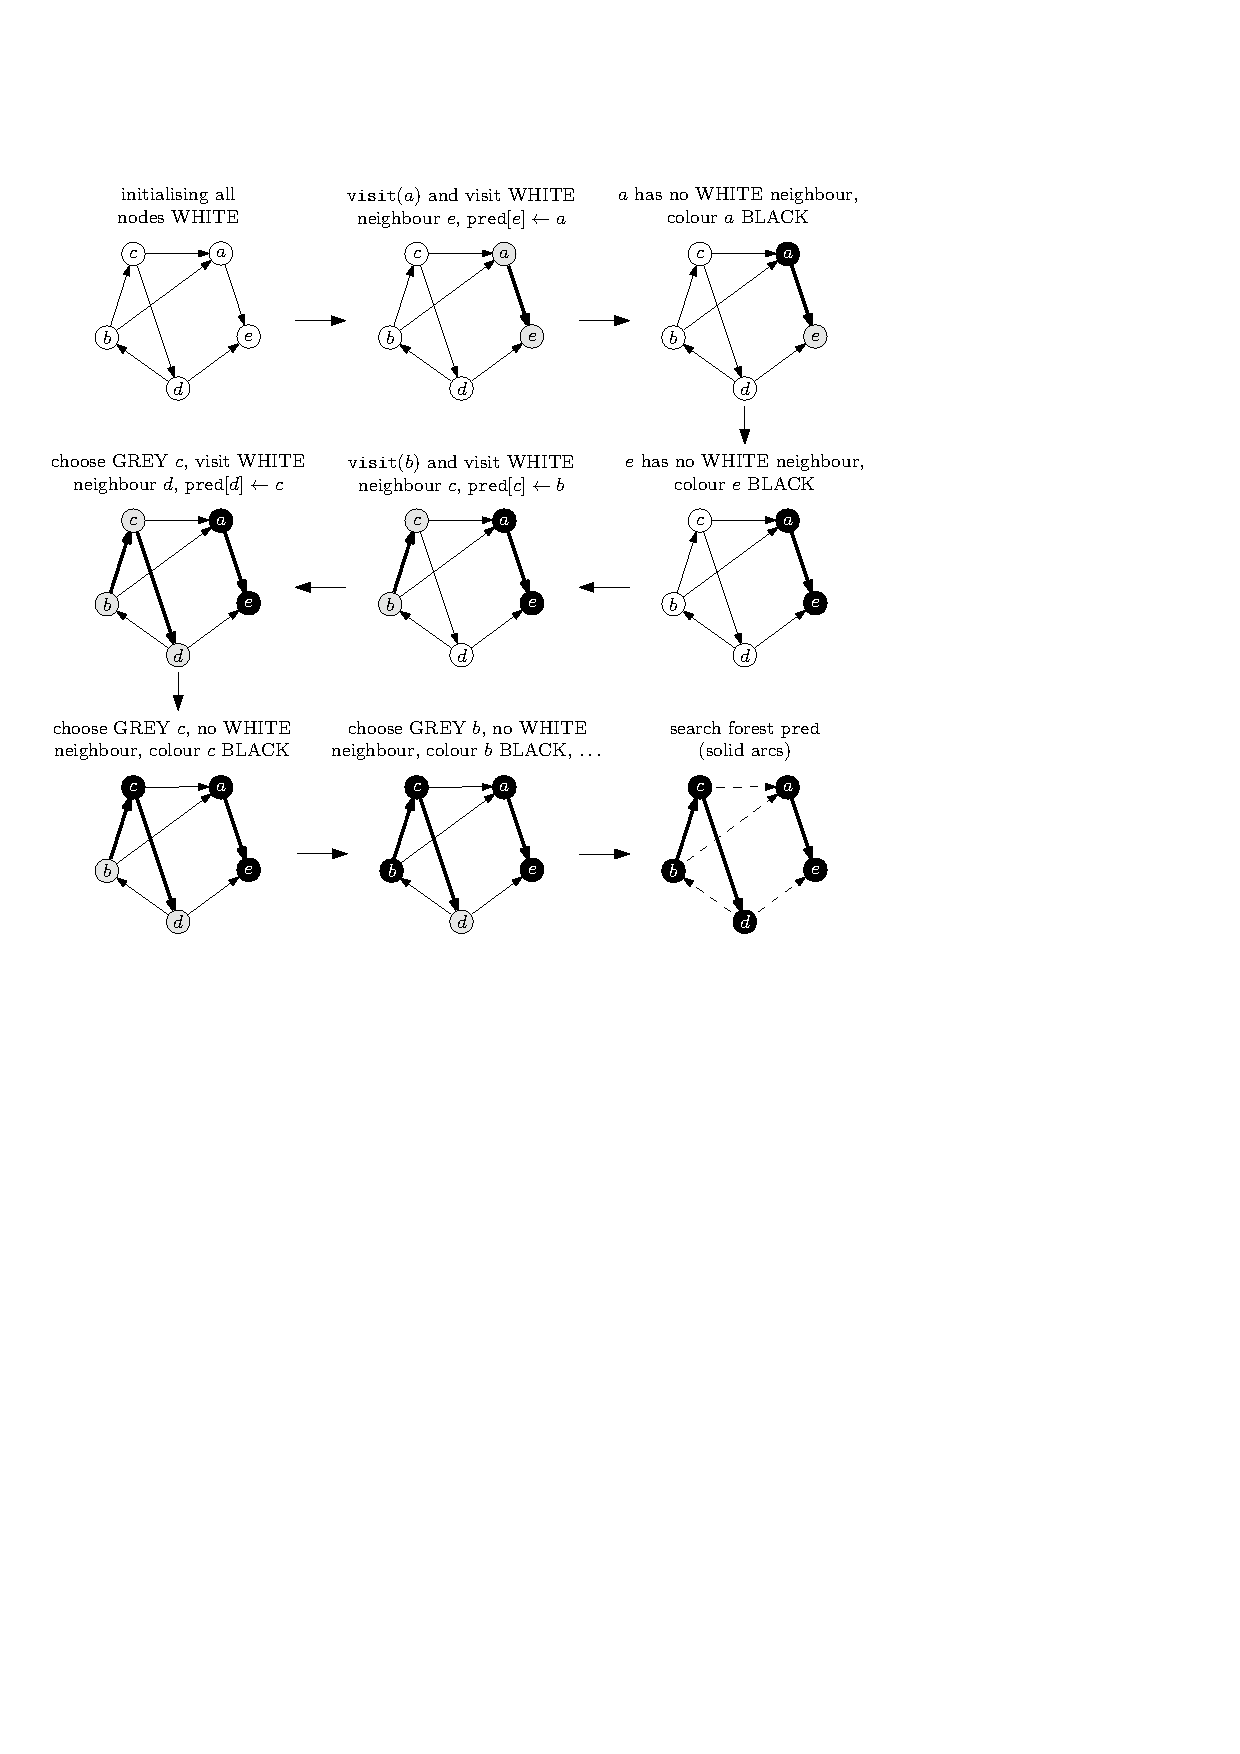
\includegraphics[width=1.0\linewidth]{traversalAlgoEx}
\end{center}
\end{Boxample}

\section{Classifying arcs after a traversal}
It helps in analysing the traversal algorithm to classify the arcs of $G$ based on their relationships in the search forest.  

\begin{Definition} \label{defn:arc-types}
Suppose we have performed a traversal of a digraph $G$, resulting in a search forest $F$. 
Let $(u, v)\in E(G)$ be an arc. Then $(u, v)$ is a
\begin{itemize} 
  \item \defnfont{tree arc} if it belongs to one of the trees of $F$;
  \item or, if it is not a tree arc, it is a
  \begin{itemize}
	\item \defnfont{forward arc} if $u$ is an ancestor of $v$ in $F$;
	\item \defnfont{back arc} if $u$ is a descendant of $v$ in $F$; 
	\item \defnfont{cross arc} if neither $u$ nor $v$ is an ancestor of the other in $F$.
  \end{itemize}
\end{itemize}
\end{Definition} 

A cross arc may join two nodes in the same tree or point from one tree to another in the search forest. 
Tree, forward and back arcs require that $u$ and $v$ be in the same tree.

\begin{Boxample}
Classify the arcs according to the definitions above. 

\begin{center}
  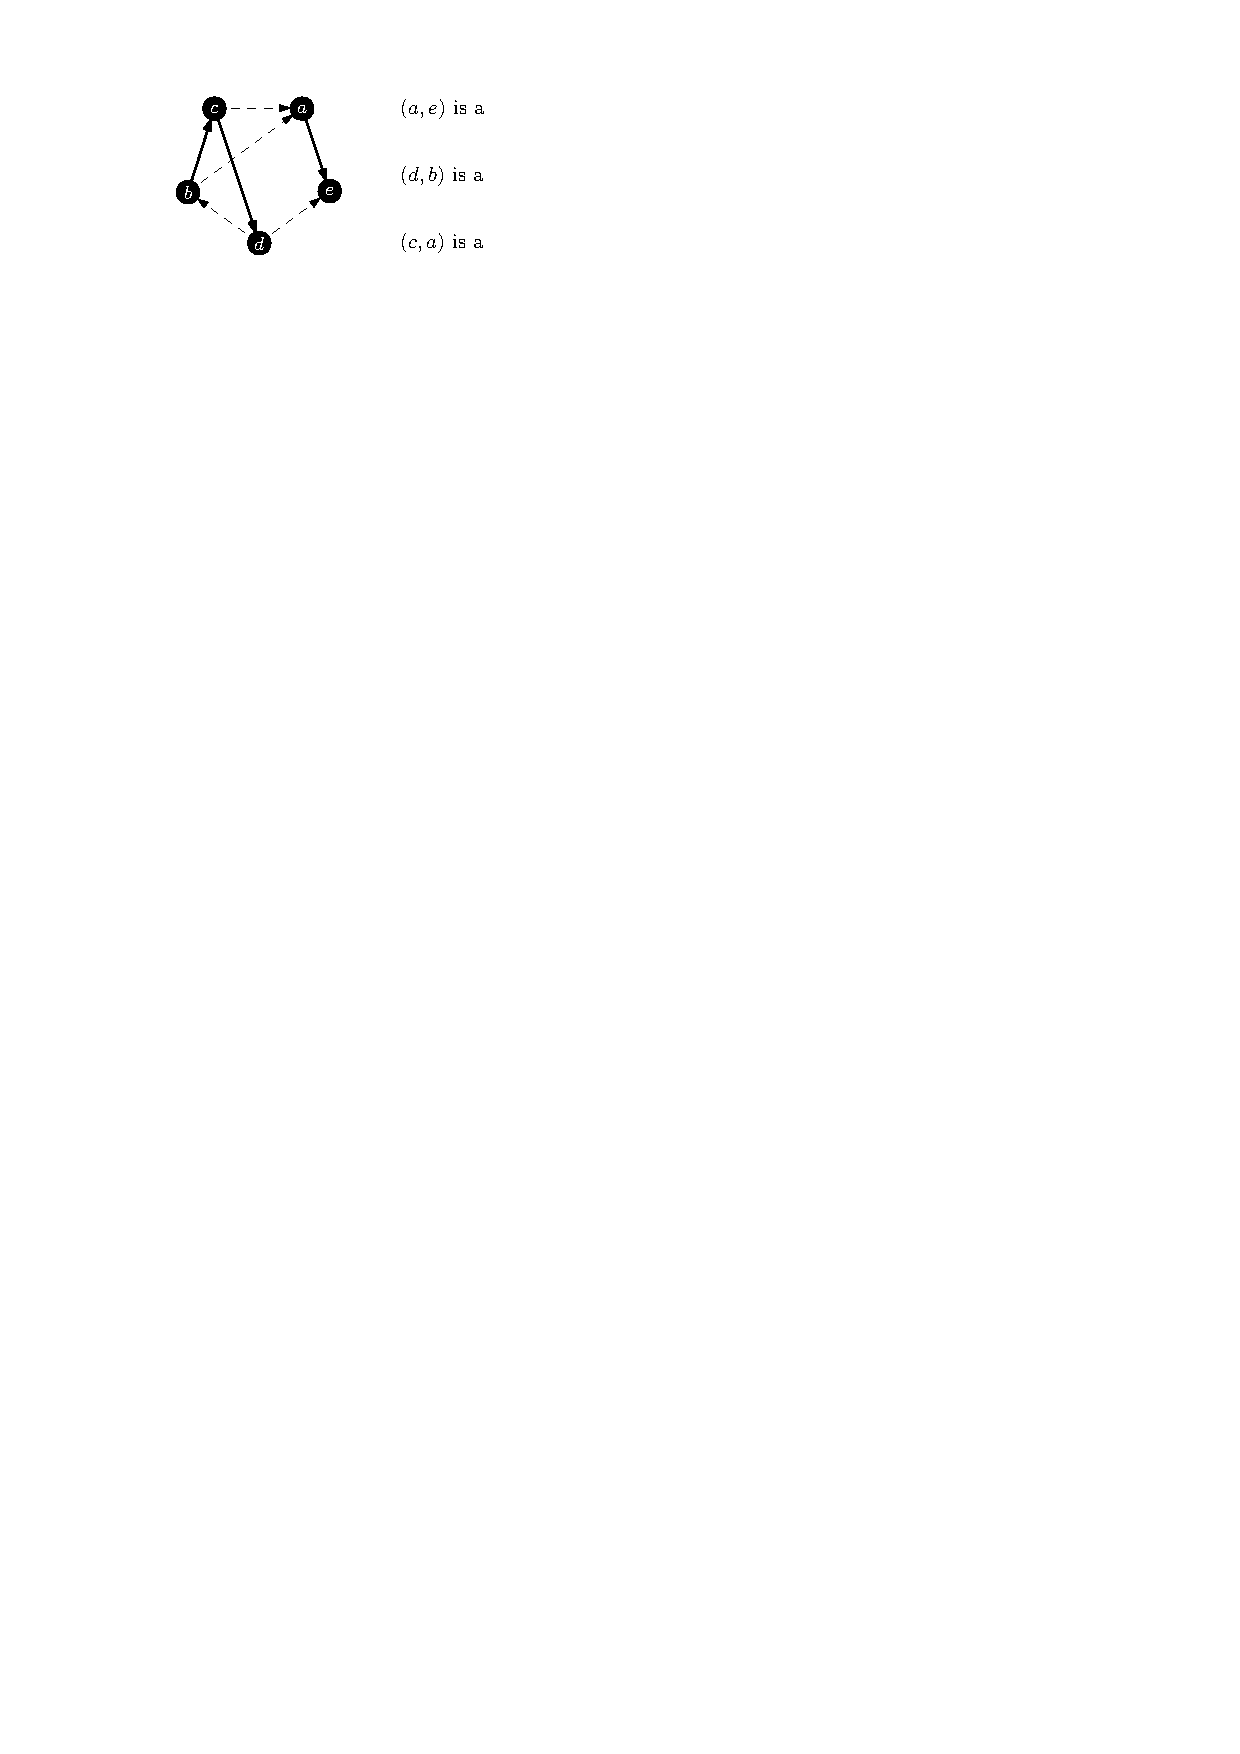
\includegraphics{traversalAlgoResultEx} 
\end{center}
\end{Boxample}

The following theorem collects all the basic facts we need for proofs
in later sections. The proofs are simple and can be done as exercises. 

\begin{Theorem} \label{thm:trav}
Suppose that we have carried out \texttt{traverse} on $G$, 
resulting in a search forest $F$. Let $v, w \in V(G)$.
\begin{itemize}
  \item Let $T_1$ and $T_2$ be different trees in $F$ and suppose that $T_1$ was explored before $T_2$. 
  Then there are no arcs from $T_1$ to $T_2$. 
  \item Suppose that $G$ is a graph. Then there can be no edges joining different trees of $F$.
  \item Suppose that $v$ is visited before $w$ and $w$ is reachable from $v$ in $G$. 
  Then $v$ and $w$ belong to the same tree of $F$.
  \item Suppose that $v$ and $w$ belong to the same tree $T$ in $F$. 
  Then any path from $v$ to $w$ in $G$ must have all nodes in $T$.
\end{itemize}
\end{Theorem}
%\begin{proof}
%If the first part were not true, then since $w$ is reachable from $v$,
%and $w$ has not been visited before $T_1$ is started, $w$ must be reached
%in the generation of $T_1$, contradicting $w\in T_2$. The second part
%follows immediately for symmetric digraphs and hence for graphs. Now
%suppose that $v$ is seen before $w$. Let $r$ be the root of the tree $T$
%containing $v$. Then $w$ is reachable from $r$ and so since it has not
%already been visited when $r$ is chosen, it belongs to $T$. Finally, if
%$v$ and $w$ are in the same tree, then any path from $v$ to $w$ in $G$
%going outside the tree must re-enter it via some arc; either the leaving
%or the entering arc will contradict the first part.
%\end{proof}

\begin{Boxample}[5]
Assuming the first statement of \cref{thm:trav}, prove the third statement.
\end{Boxample}

\section{Running time for the general traversal algorithm}
The generality of our traversal algorithm makes it exact running time impossible to determine.  
It depends on how one chooses the next grey node $u$ and its white neighbour $v$.  
Some schemes for choosing $u$ and $v$ can be complex and depend on $n$. 
The schemes we consider here are simple and constant time.

% It also apparently depends on how long it takes to determine 
% whether there exist any grey nodes or whether $u$ has any white neighbours. 
% However, any sensible rule for checking existence of either type of node 
% should simply return false if there is no such node, 
% and take no more time in this case than if it does find one. 
% Thus we do not need to take account of the checking in our analysis.

\begin{itemize}
  \item The initialization of the array $\colour$ takes time $\Theta(n)$ so \texttt{traverse} 
  is in $\Theta(n + t)$, where $t$ is the total time taken by all the calls to \texttt{visit}.
  \item We execute the while-loop of \texttt{visit} in total $\Theta(n)$ times 
  since every node must eventually move from white through grey to black. 
  \item The time taken in choosing grey nodes is $\Omega(n)$. 
  \item The time taken to find a white neighbour involves examining each neighbour of $u$ 
  and checking whether it is white, then applying a selection rule. 
  \item The total time in choosing white neighbours is in $\Omega(m)$ if adjacency lists are used 
  and is in $\Omega(n^2)$ if an adjacency matrix is used.
  \item So the running time of \texttt{traverse} is $\Omega(n + (n+m)) = \Omega(n + m)$
  if adjacency lists are used, and $\Omega(n + n^2) = \Omega(n^2)$ if the adjacency matrix format is used.
\end{itemize}

So for simple selection rules and assuming a sparse input digraph, the adjacency list format seems
preferable. But if more complex selection rules are used, for example, choosing a single grey node is 
of order $n$ while choosing a single white node is still constant time, then the running time is 
asymptotically $\Omega(n^2)$ regardless of the data structure, so using
the adjacency matrix is not clearly ruled out.


\chapter{Depth first search (DFS)} %------------------------------------------------
Traversal algorithms differ in the rules for choosing the next grey and next white node, 
with different rules leading to very different results.

\begin{Definition}
In \defnfont{depth-first search} (DFS) the new grey node chosen is the one
that has been grey for the \boldfont{shortest} time.
\end{Definition}

DFS takes us away from the root node as quickly as possible. 
If the first visited neighbour of the root has a neighbour, we immediately visit that neighbour. 
Then, if that has a neighbour, we visit that and so on, thus ``deeply'' searching as far away from the root as possible. 
We backtrack as little as possible before continuing away from the root again. The root is the last node to turn black.

There still remains the choice of which white neighbour of the chosen grey node to visit. 
It does not matter what choice is made but our \boldfont{convention is to choose the one with
lowest index} (recall that nodes have indices $0, \dots, n - 1$). 

These choices can be made in constant time so that the running time is  $\Omega(n + m)$ (assuming adjacency lists) 
and DFS is linear in the size $+$ order of a digraph. 

\begin{Boxample}[2]
A digraph and its DFS search tree, rooted at node $0$. The dashed arcs indicate the original arcs that are not part of the DFS search tree.
\begin{center}
  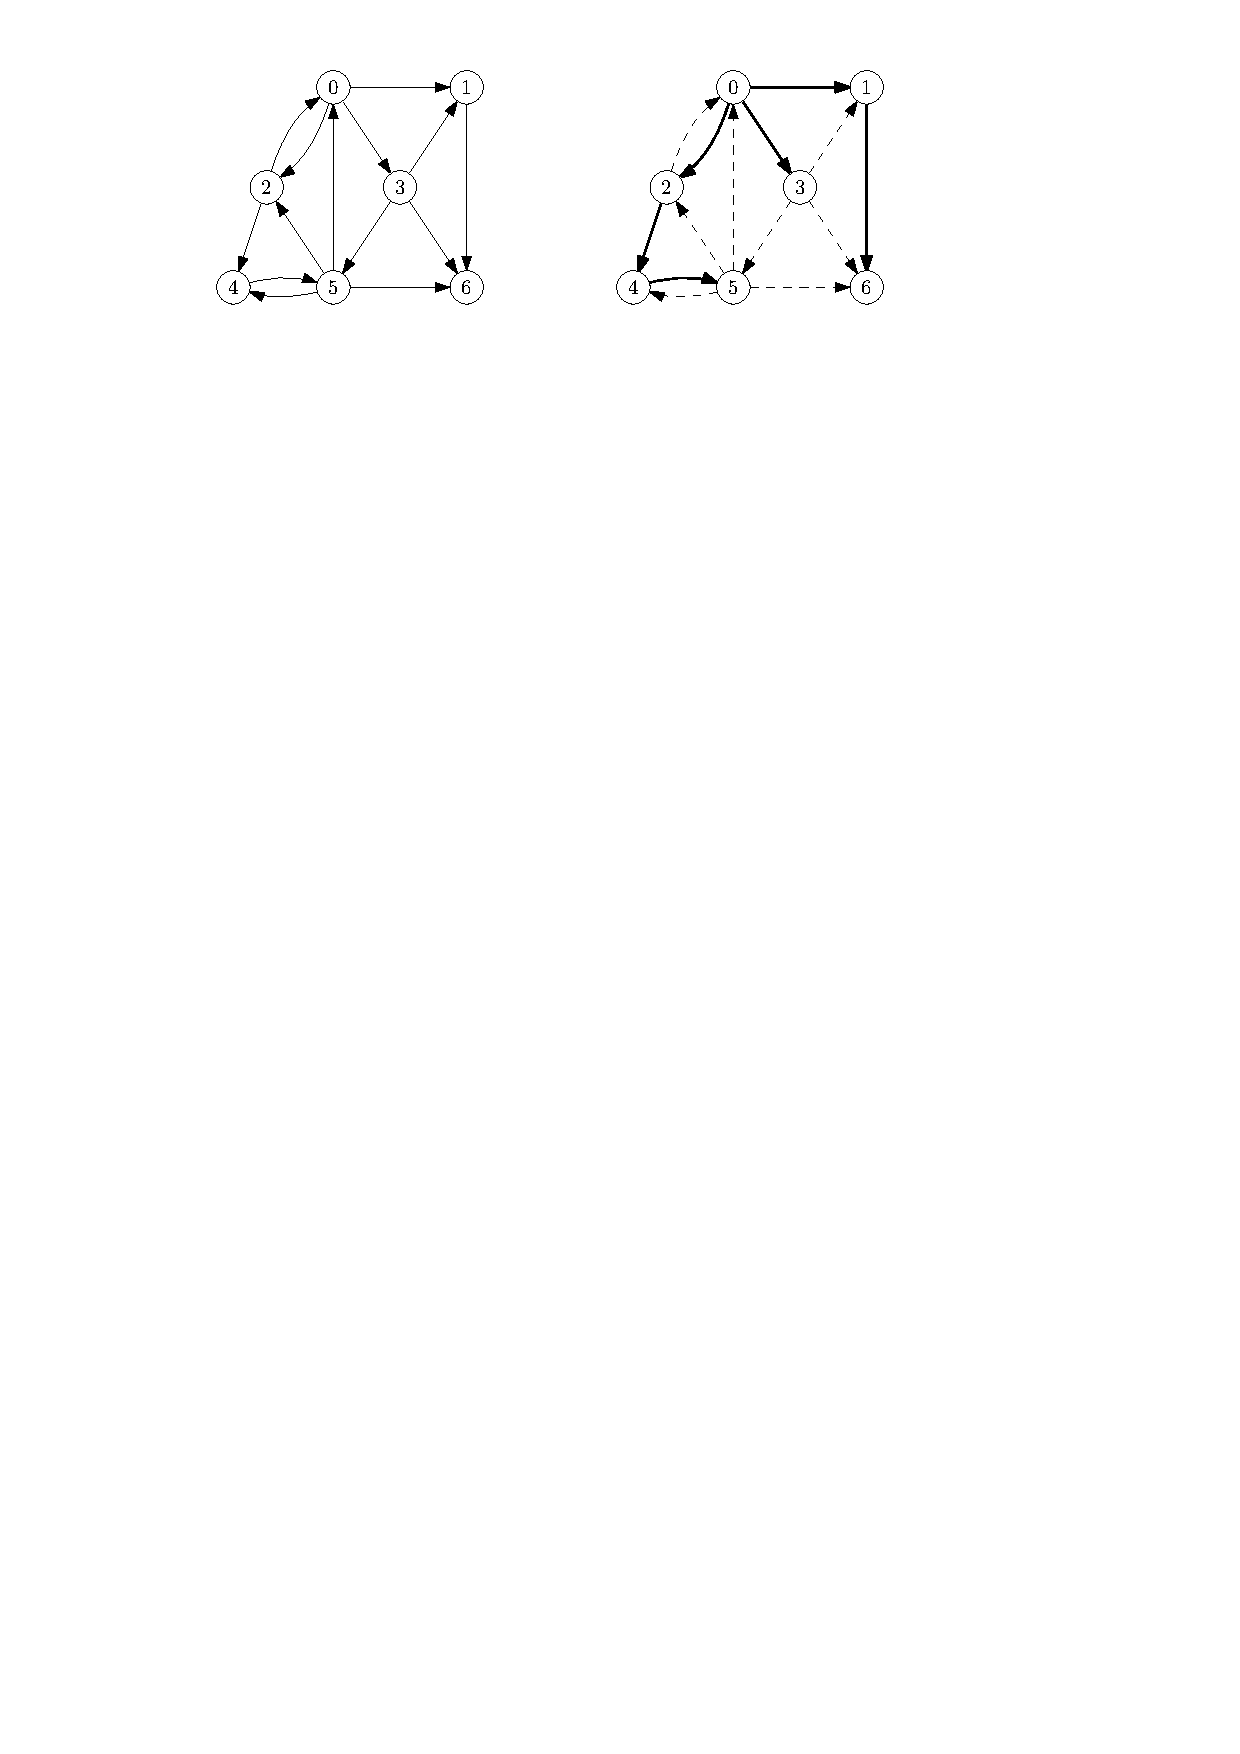
\includegraphics{DFSalgoDigraph}
\end{center}
Find a tree arc, cross arc, forward arc and back arc (or say if that type of arc does not exist for that traversal).
\end{Boxample}

\begin{Boxample}[2]
Use the nodes on the right to draw the search tree you obtain by running DFS on the graph on the left, starting at vertex $0$. 
Use dashed edges to indicate edges that are not arcs in the search tree.
\begin{center}
  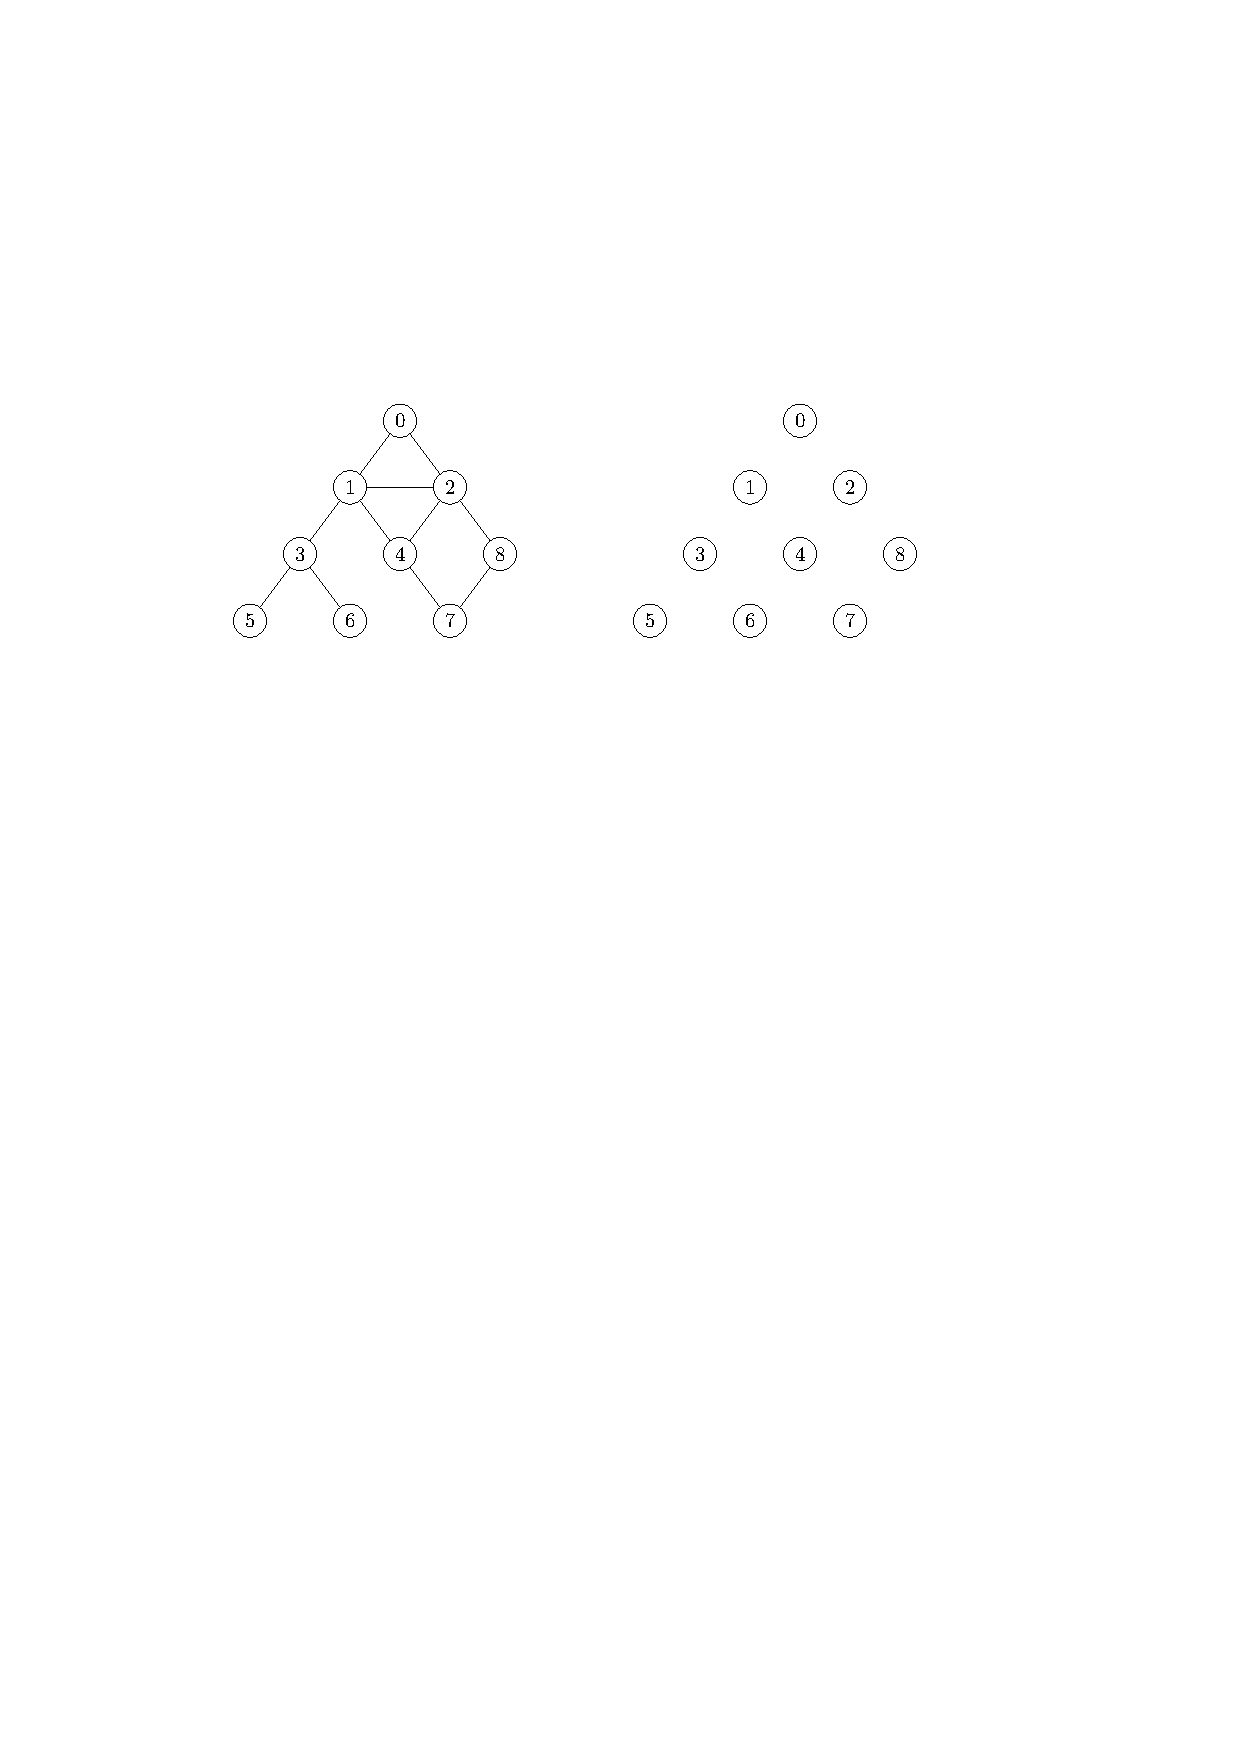
\includegraphics{TraverseGraphEx} 
\end{center}
Find a tree arc, cross arc, forward arc and back arc (or say if that type of arc does not exist for that traversal).
\end{Boxample}

For a general digraph, and unlike the examples given here, all nodes may not be reachable from the starting node. 
In this case, we get a search forest where the number of trees in the forest is the number of calls made to \texttt{DFSvisit}.

\section{Pseudocode for depth-first search} \label{ss: DFS}
The ``last in, first out" order of choosing grey nodes in DFS is mimicked by a \boldfont{stack} data structure. 
We thus store grey nodes in a stack as they are discovered. 

The pseudocode for \algfont{DFS} and \algfont{DFSvisit} is in \cref{alg:DFScode,alg:DFSvisitcode}. 
\begin{itemize}
  \item We loop through the nodes adjacent to the chosen grey node $u$, 
  and as soon as we find a white one, we add it to the stack.
  \item We also introduce a variable $\timeVar$ and keep track of the time a node changes colour
  \item The array $\seen$ records the time a node turns grey
  \item The array  $\done$ records the time a node turns black
\end{itemize}

\begin{algorithm}[H]
  \caption{Depth-first search algorithm.}
    \label{alg:DFScode}
\begin{algorithmic}[1]
\Function{DFS}{digraph $G$}
	\State stack $S$ 
	\State array $\colour[0..n-1]$, $\pred[0..n-1]$, $\seen[0..n-1]$, $\done[0..n-1]$
	\For{$u \in V(G)$}  
		\State $\colour[u] \gets $ WHITE; $\pred[u] \gets $ \texttt{null} \Comment{initialise arrays}
	\EndFor
	\State $\timeVar \gets 0$ \Comment{time will increment at every node colour change}
	\For{$s \in V(G)$} 
		\If{$\colour[s] = $ WHITE}  \Comment{find a WHITE node}
			\State \texttt{DFSvisit}$(s)$ \Comment{start traversal from $s$}
		\EndIf
	\EndFor
	\State \Return{$\pred, \seen, \done$}
\EndFunction
\end{algorithmic}
\end{algorithm}

\begin{algorithm}[H]
  \caption{Depth-first visit algorithm.}
    \label{alg:DFSvisitcode}
\begin{algorithmic}[1]
\Function{DFSvisit}{node $s$}
	\State $\colour[s] \gets $ GREY 
	\State $\seen[s] \gets \timeVar$; $\timeVar \gets \timeVar + 1$
	\State $S$.\texttt{insert}$(s)$ \Comment{put $s$ in stack}
	\While{\textbf{not} $S$.\texttt{isEmpty}$()$}
		\State $u \gets S$.\texttt{peek}$()$  \Comment{get node at front of stack}
		\If{there is a neighbour $v$ with $\colour[v] = $ WHITE}
			\State $\colour[v] \gets $ GREY; $\pred[v] \gets u$  \Comment{visit neighbour, update tree}
			\State $\seen[v] \gets \timeVar$; $\timeVar \gets \timeVar + 1$  \Comment{record and increment time}
			\State $S$.\texttt{insert}$(v)$  \Comment{put neighbour in stack}
		\Else
			\State $S$.\texttt{delete}$()$  \Comment{delete node from stack}
			\State $\colour[u] \gets $ BLACK  \Comment{colour it done}
			\State $\done[u] \gets \timeVar$; $\timeVar \gets \timeVar + 1$  \Comment{record and increment time}
		\EndIf
	\EndWhile
\EndFunction
\end{algorithmic}
\end{algorithm}

Given the relationship between stacks and recursion, we can replace the \texttt{DFSvisit} procedure by
a recursive version \algfont{recursiveDFSvisit}: 

\begin{algorithm}[H]
  \caption{Recursive DFS visit algorithm.}
    \label{alg:DFSreccode}
\begin{algorithmic}[1]
\Function{recursiveDFSvisit}{node $s$}
	\State $\colour[s] \gets $ GREY \
	\State $\seen[s] \gets \timeVar$; $\timeVar \gets \timeVar + 1$
	\For{each $v$ adjacent to $s$}
		\If{$\colour[v] = $ WHITE} \Comment{each unvisited neighbour}
			\State $\pred[v] \gets s$ \Comment{update tree}
			\State \texttt{recursiveDFSvisit}$(v)$ \Comment{now visit neighbour}
		\EndIf
	\EndFor
	\State $\colour[s] \gets $ BLACK \Comment{visted all white neighbours so done}
	\State $\done[s] \gets \timeVar $; $\timeVar \gets \timeVar + 1$
\EndFunction
\end{algorithmic}
\end{algorithm}

\begin{Boxample}
jo TODO: this and the equiavlent BFS example are great. How about another one with just the first full grpah, nodes elsewhere and empty seen/done boxes arrays the epolpe can fill out themselves?

DFS with \texttt{recursiveDFSvisit}. 
\begin{center}
  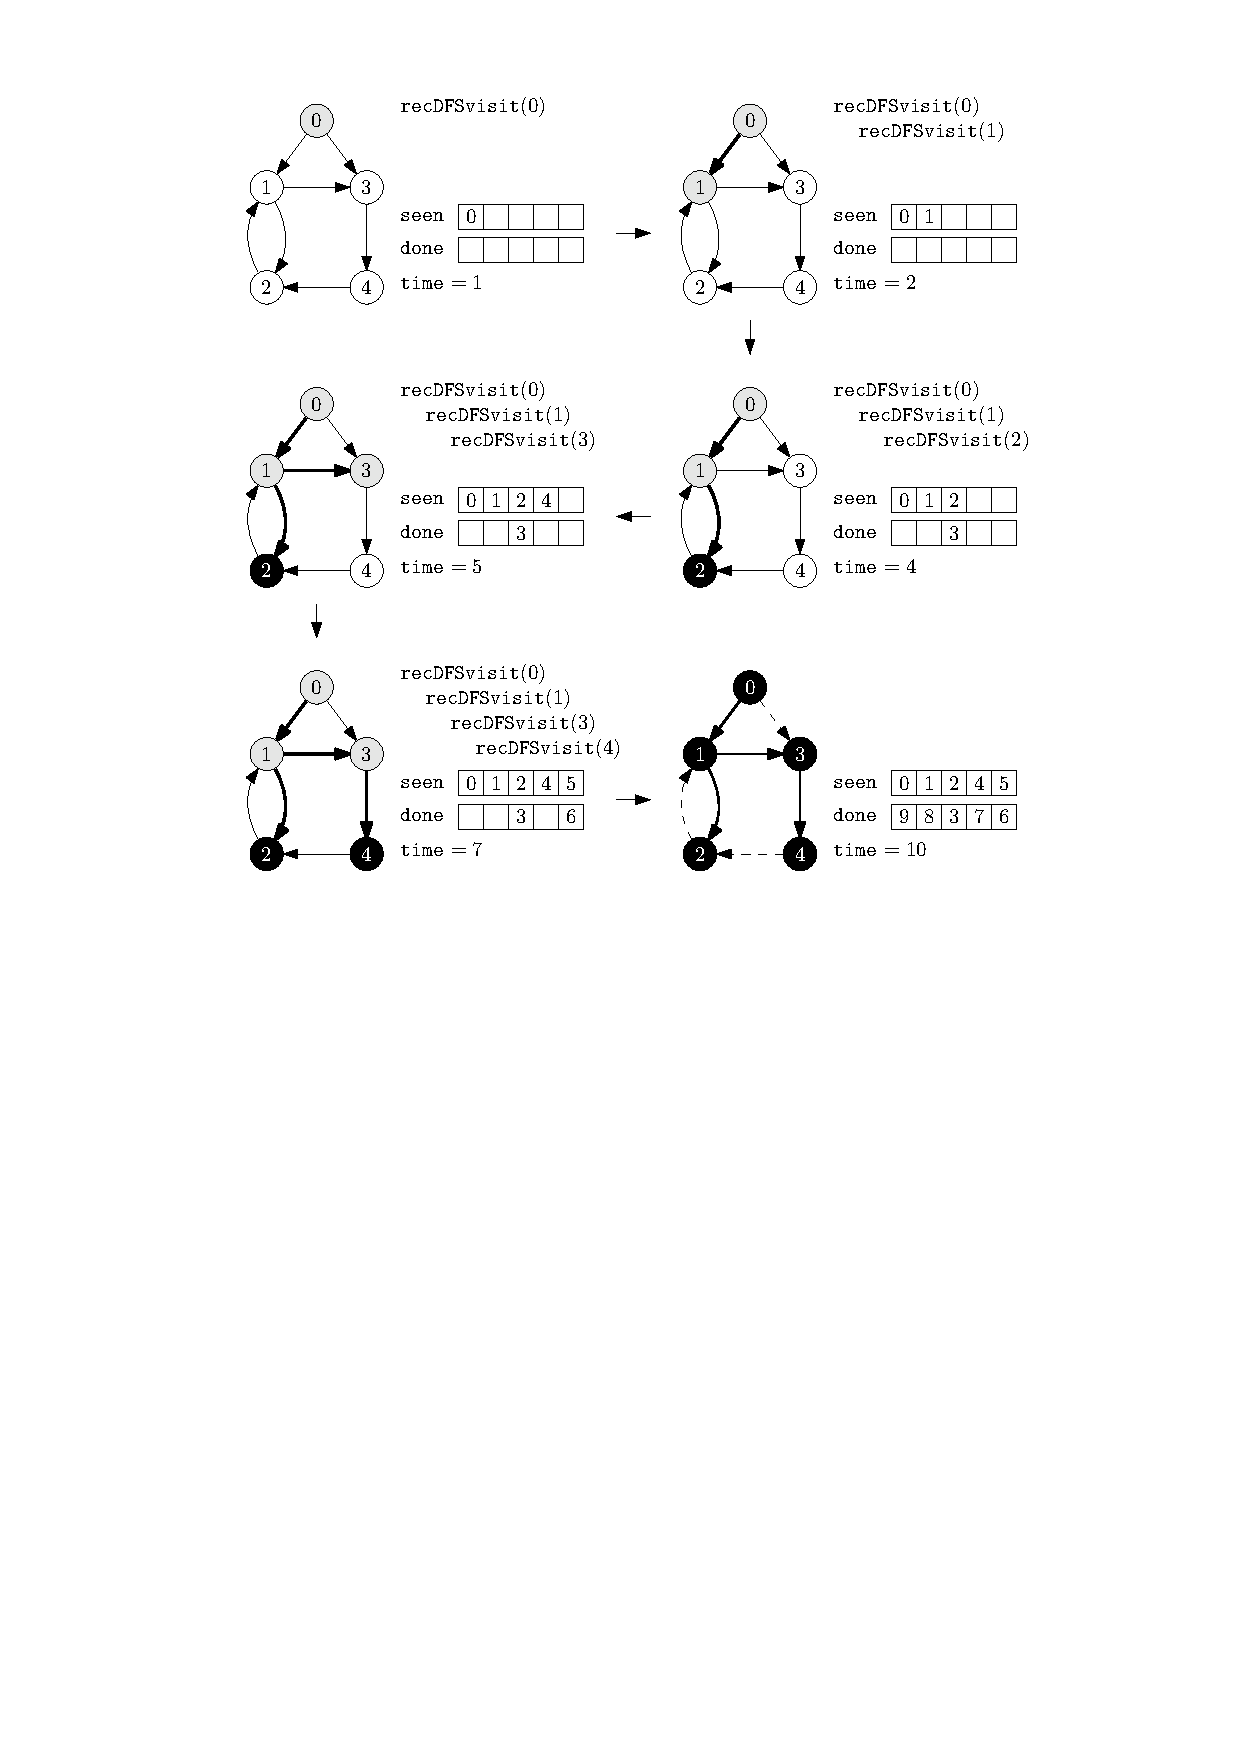
\includegraphics[width=1.0\linewidth]{DFSalgoRecursive2}
\end{center}
\end{Boxample}

\section{DFS useful results and facts}
\begin{Theorem}
\label{thm:DFS-seen-done}
Suppose that we have performed DFS on a digraph $G$, resulting in a 
search forest $F$. Let $v, w \in V(G)$ and suppose that $\seen[v] < \seen[w]$. 

\begin{itemize}
\item
If $v$ is an ancestor of $w$ in $F$, then 
$$\seen[v] < \seen[w] < \done[w] < \done[v].$$
\item
If $v$ is not an ancestor of $w$ in $F$, then
$$\seen[v] < \done[v]  < \seen[w] < \done[w].$$
\end{itemize}
\end{Theorem}
%\begin{proof} The first part is clear from the recursive formulation
%of DFS. Now suppose that $v$ is not an ancestor of $w$. Note that $w$
%is obviously also not an ancestor of $v$. 
%%Let $x$ be the root of the tree of $F$ containing $v$. 
%Thus $v$ lives in a subtree that is completely explored before the 
%subtree of $w$ is visited by \texttt{recursiveDFSvisit}.
%\end{proof}

Note that this result rules out  the timestamps $\seen[v] < \seen[w] < \done[v] < \done[w]$.

All four types of arcs in our search forest classification can
arise with DFS. The different types of arcs can be easily
distinguished while the algorithm is running or by looking at the timestamps 
$\seen$ and $\done$.

\begin{Boxample}[5]
Explain how to determine, at the time when an arc is first explored by
\texttt{DFS}, whether it is a tree-, back-, forward- or cross-arc.
\end{Boxample}

\begin{Boxample}[5] \label{ex:DFS-arc-class}
Suppose that we have performed \texttt{DFS} on a digraph $G$.
 Let $(v, w)\in E$. The following statements are true. Prove the first statement.
\begin{itemize}
  \item $(v, w)$ is a tree or forward arc if and only if  
	$$\seen[v] < \seen[w] < \done[w] < \done[v]\text{;}$$
  \item $(v, w)$ is a back arc if and only if
	$$\seen[w] <  \seen[v] < \done[v] < \done[w]\text{,}$$ 
  \item $(v, w)$ is a cross arc if and only if 
	$$\seen[w] < \done[w]  < \seen[v] < \done[v]\text{.}$$
\end{itemize}
\end{Boxample}

%\begin{Boxample}[3] \label{ex:DFS-graph-no-cross}
%Suppose that DFS is run on a graph $G$. Prove that cross edges do not occur.
%\end{Boxample}


\chapter{Breadth First Search (BFS) and Priority\\ First Search (PFS)} %------------------
\begin{Definition}
In \defnfont{breadth-first search} (BFS) the new grey node chosen is the one
that has been grey for the \boldfont{longest} time
\end{Definition}
 
BFS takes us away from the root node as slowly as possible. 
First we visit the root, then all its neighbours, then all neighbours of its neighbours and so on. 
The root is the first node to turn black.

As with DFS, the running time of BFS is in $\Theta(n+m)$ when implemented using adjacency lists.

\begin{Boxample}[4]
A digraph and its BFS search tree, rooted at node $0$. 
The dashed arcs indicate the original arcs that are not part of the BFS search tree.
\begin{center}
  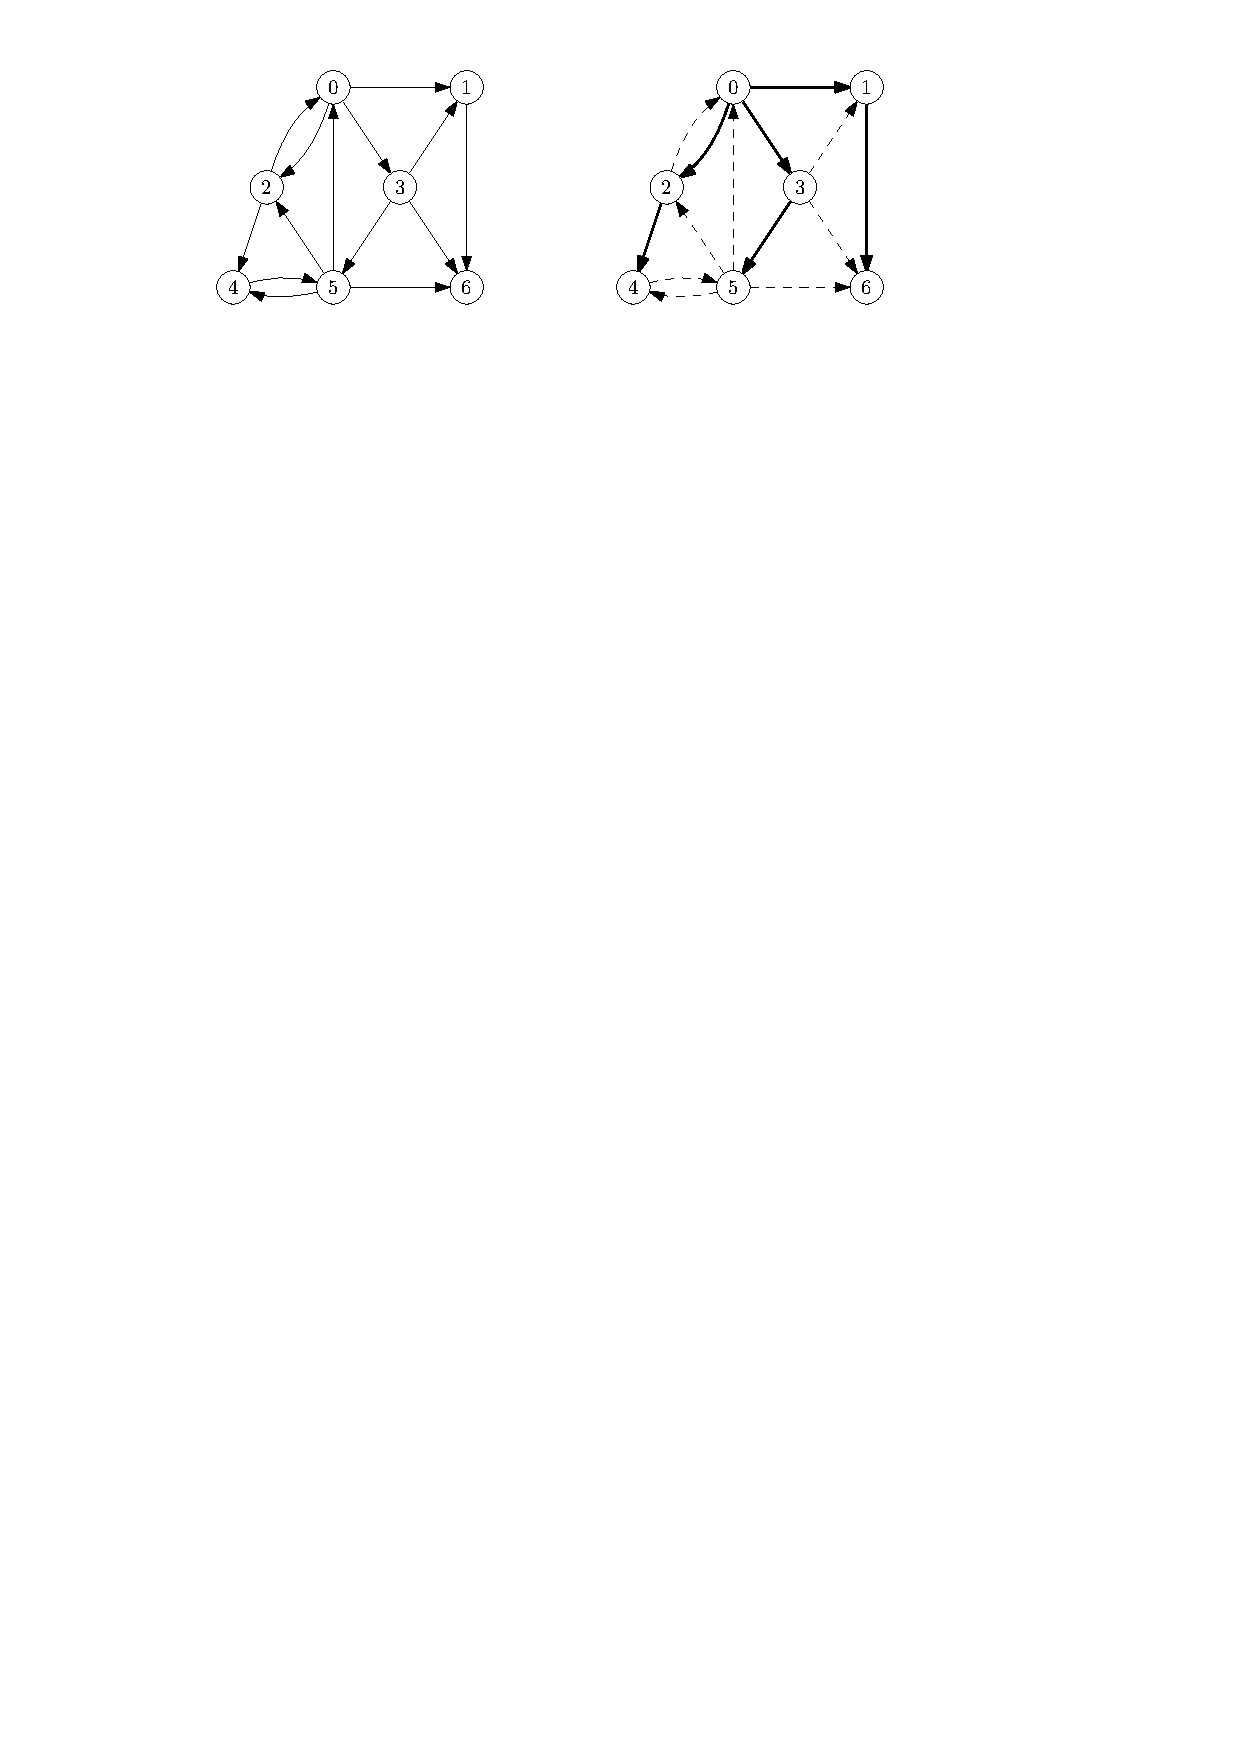
\includegraphics{BFSalgoDigraph} 
\end{center}
Find a tree arc, cross arc, forward arc and back arc (or say if that type of arc does not exist for that traversal).
\end{Boxample}

\begin{Boxample}[2]
Use the nodes on the right to draw the search tree you obtain by running BFS on the graph on the left, starting at vertex $0$. 
Use dashed edges to indicate edges that are not arcs in the search tree.
\begin{center}
  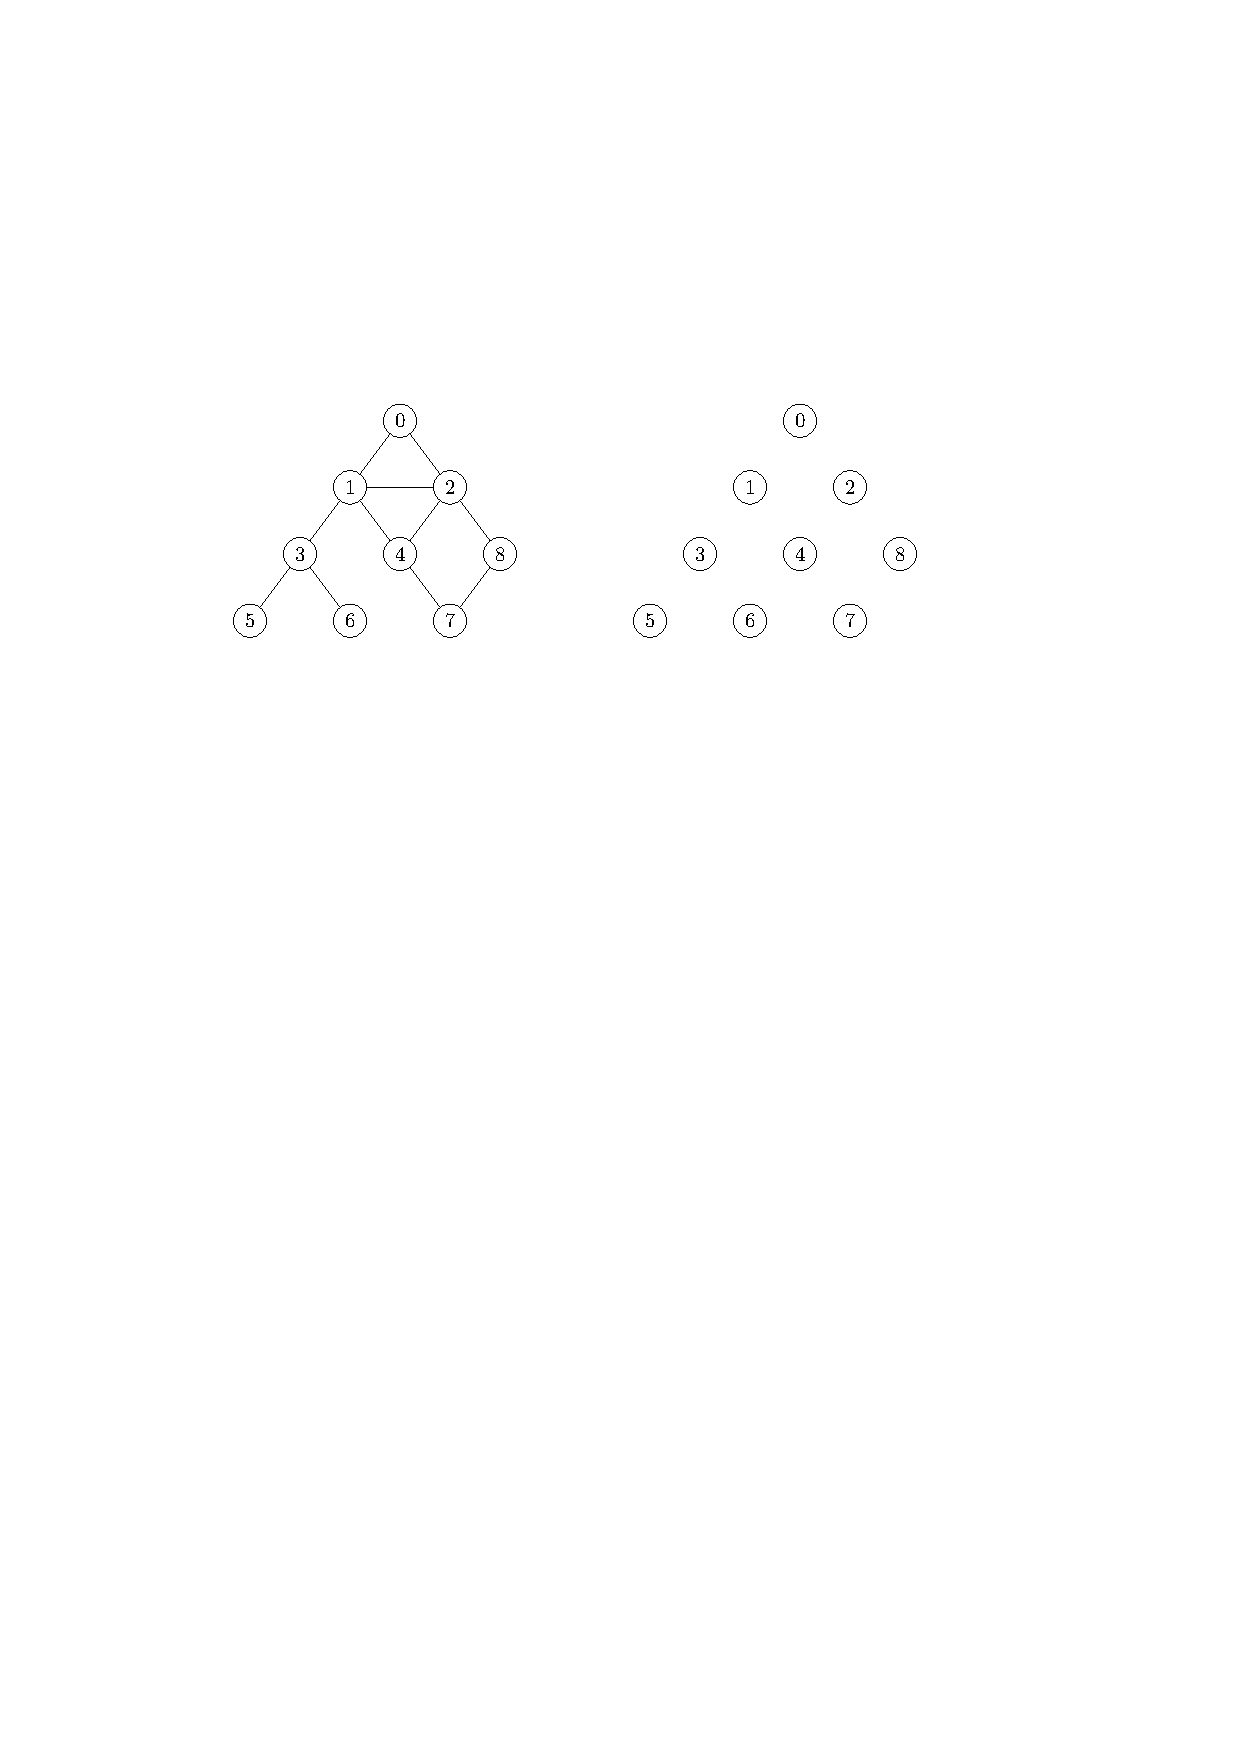
\includegraphics{TraverseGraphEx}
\end{center}
Find a tree arc, cross arc, forward arc and back arc (or say if that type of arc does not exist for that traversal).
\end{Boxample}
 
\section{Pseudocode for breadth-first search} \label{sec:bfs}
The first-in first-out processing of the grey nodes in BFS is ideally handled by a queue. 
The pseudocode for \algfont{BFS} and \algfont{BFSvisit} is in \cref{alg:BFScode,alg:BFSvisitcode}.
The time\-stamps $\seen$ and $\done$ of DFS are of less use here. 
It is more useful to record the number of steps from the root in the array $d$.

\begin{algorithm}[H]
  \caption{Breadth-first search algorithm.}
    \label{alg:BFScode}
\begin{algorithmic}[1]
\Function{BFS}{digraph $G$}
	\State queue $Q$  
	\State array $\colour[0..n-1]$, $\pred[0..n-1]$, $d[0..n-1]$
	\For{$u \in V(G)$} 
		\State $\colour[u] \gets $ WHITE; $\pred[u] \gets $ \texttt{null}
	\EndFor
	\For{$s \in V(G)$} 
		\If{$\colour[s] = $ WHITE } 
			\State \texttt{BFSvisit}$(s)$
		\EndIf
	\EndFor
	\State \Return{$\pred, d$}
\EndFunction
\end{algorithmic}
\end{algorithm}

\begin{algorithm}[H]
  \caption{Breadth-first search visit algorithm.}
     \label{alg:BFSvisitcode}
  \begin{algorithmic}[1]
\Function{BFSvisit}{node $s$}
	\State $\colour[s] \gets $ GREY; $d[s] \gets 0$ 
	\State $Q$.\texttt{insert}$(s)$
	\While{\textbf{not} $Q$.\texttt{isEmpty}$()$}
		\State $u \gets Q$.\texttt{peek}$()$
		\For{each $v$ adjacent to $u$}
			\If{$\colour[v] = $ WHITE}
				\State $\colour[v] \gets $ GREY; $\pred[v] \gets u$; $d[v] \gets d[u]+1$
				\State $Q$.\texttt{insert}$(v)$
			\EndIf
		\EndFor
		\State $Q$.\texttt{delete}$()$
		\State $\colour[u] \gets $ BLACK
	\EndWhile
\EndFunction
\end{algorithmic}
\end{algorithm}

\begin{Boxample}
jo TODO: see request in DFS boxample. Would be good to get another of these that students can do in class.
BFS on a digraph.
\begin{center}
  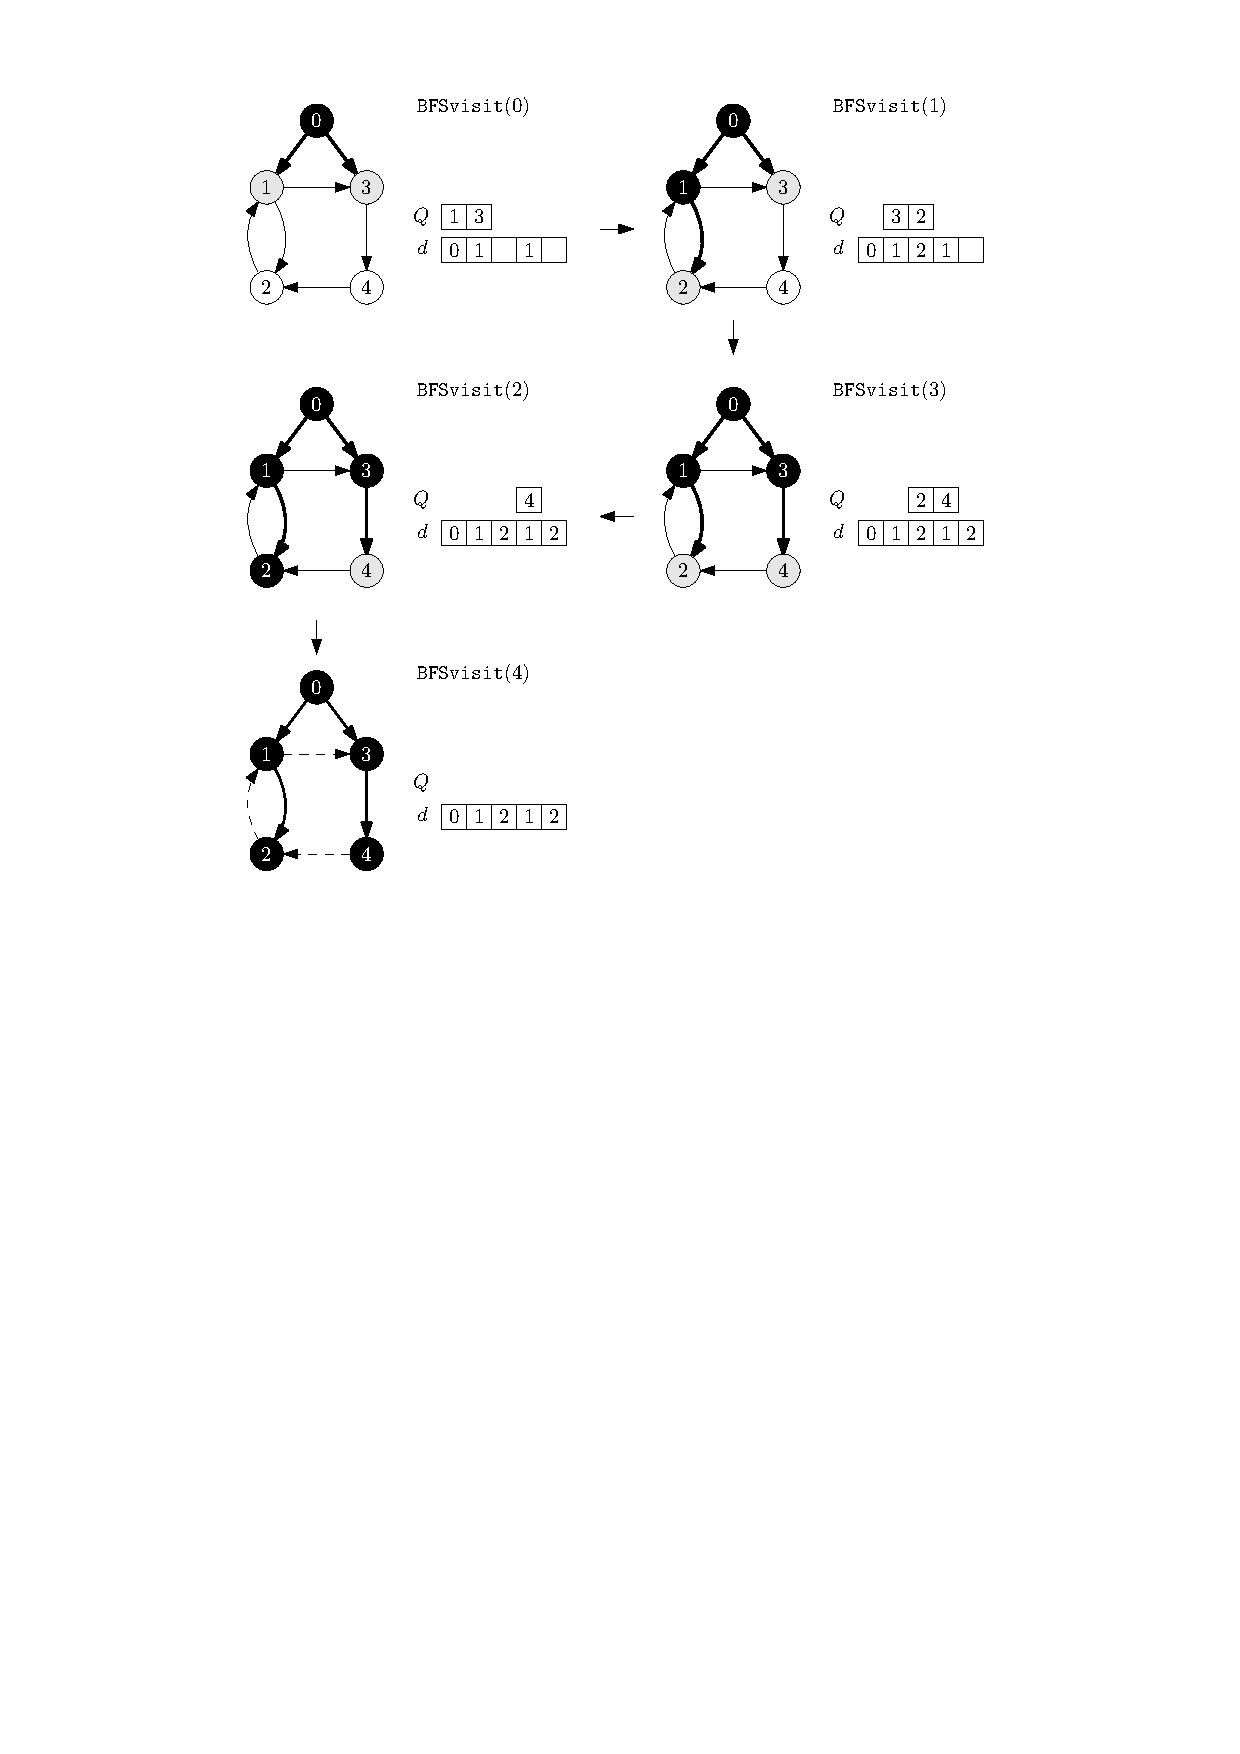
\includegraphics{BFSalgoQueue2}
\end{center}
\end{Boxample}

\section{BFS useful results and facts} 
It is rather obvious that BFS processes all nodes at distance 1, then
all nodes at distance 2, etc, from the root. 
The formal theorem stating this is given below without proof (see book for a simple inductive proof).

\begin{Theorem} \label{thm:BFSdist}
Suppose we run \texttt{BFS} on a digraph $G$.
Let $v \in V(G)$, and let $r$ be the root of the search tree containing $v$. 
Then $d[v] = d(r, v)$.
\end{Theorem}

We can classify arcs, but the answer is not as nice as with DFS.

\begin{Theorem} \label{thm:BFS-arcclass}
Suppose that we are performing \texttt{BFS} on a digraph $G$. Let $(v,
w)\in E(G)$ and suppose that we have just chosen the grey node $v$. 
Then
\begin{itemize}
  \item if $(v, w)$ is a tree arc then $\colour[w] = $ WHITE, $d[w] = d[v] + 1$;
  \item if $(v, w)$ is a back arc, then $\colour[w] = $ BLACK, $d[w] \leq d[v] - 1$;  
  \item there are no forward arcs; and
  \item if $(v, w)$ is a cross arc then one of the following holds:
  \begin{itemize}
	\item $d[w] < d[v] - 1$, and $\colour[w] = $ BLACK;
	\item $d[w] = d[v]$, and $\colour[w] = $ GREY;
	\item $d[w] = d[v]$, and $\colour[w] = $ BLACK;
	\item $d[w] = d[v] - 1$, and $\colour[w] = $ GREY;
	\item $d[w] = d[v] - 1$, and $\colour[w] = $ BLACK.
  \end{itemize}
\end{itemize}
\end{Theorem}

\begin{Boxample}[6]
Explain why there are no forward arcs when performing BFS on a digraph.
\end{Boxample}

%\begin{proof}
%The arc is added to the tree if and only if $w$ is white. If the arc is
%a back arc, then $w$ is an ancestor of $v$; the FIFO queue structure
%means $w$ is black before the adjacency list of $v$ is scanned. 
%
%Now suppose that $(x, u)$ is a forward arc. Then since $u$ is a
%descendant of $x$ but not a child in the search forest, 
%Theorem~\ref{thm:BFSdist} yields $d[u]
%\geq d[x] + 2$. But by the last theorem we have $d[u] = d(s, u) \leq
%d(s, x) + 1 = d[x] + 1$, a contradiction. Hence no such arc exists.
%
%A cross arc may join two nodes on the same level, jump up one level,
%or jump up more than one level. In the last case, $w$ is already black
%before $v$ is seen. In the second case, $w$ may be seen before $v$,
%in which case it is black before $v$ is seen (recall $w$ is not the
%parent of $v$), or it may be seen after $v$, in which case it is grey
%when $(v, w)$ is explored. In the first case, $w$ may be seen before $v$ (in
%which case it is black before $v$ is seen), or $w$ may be seen after $v$
%(in which case it is grey when $(v, w)$ is explored).
%\end{proof}

In the special case of graphs we can say more.

\begin{Theorem} \label{thm:BFS-grapharcclass}
Suppose that we have performed \texttt{BFS} on a graph $G$. 
Let $\{v, w\}\in E(G)$. Then exactly one of the following conditions holds.
\begin{itemize}
	\item $\{v, w\}$ is a tree edge, $| d[w] - d[v] |= 1$;
	\item $\{v, w\}$ is a cross edge, $d[w] = d[v]$;
	\item $\{v, w\}$ is a cross edge, $| d[w] - d[v] | = 1$.
\end{itemize}
\end{Theorem}
%\begin{proof} By Theorem~\ref{thm:BFS-arcclass} there can be no forward
%edges, hence no back edges. A cross edge may not jump up more than
%one level, else it would also jump down more than one level, which is
%impossible by Theorem~\ref{thm:BFSdist}.
%\end{proof}

% For a given BFS tree, we can uniquely label the vertices of a digraph based on the time they were first seen. 
% For the graph $G_1$ of \cref{fig:graphExample2}, we label vertex 0 with 1,
% vertices \set{1,2} with labels \set{2,3}, vertices \set{3,4,8} with labels \set{4,5,6}, 
% and the last vertex level \set{5,6,7} with labels \set{7,8,9}.  
% These are indicated in \cref{fig:graphEx2-BFS}.

\section{Priority-first search} \label{sec:PFS}
Priority-first search is a more general and sophisticated form of traversal that encompasses both BFS and DFS (and others). 

\begin{itemize}
	\item Each grey node has associated with it an integer \defnfont{key}. 
	\item The interpretation of the key is of a priority: 
	the smaller the key, the higher the priority. 
	\item The rule for choosing a new grey node is to choose one with the smallest key.  
	\item The key can either be assigned once when the node is first seen and then left unchanged, 
	or could be updated at other times. We concentrate on unchanging keys here.
	\item To mimic BFS, set the key for the node $v$ to be the time that $v$ turns grey. 
	It will always remain as the lowest key until it turns black.
	\item To mimic DFS, set the key for node $v$ to be $-\seen[v]$, 
	so that the most recently seen node has the lowest key
	\item The running time of PFS depends on how long it takes to find the minimum key value.
	\item The rules described here implemented using an array take $\Omega(n)$ to find the lowest key 
	so the algorithm is $\Theta(n^2)$. Contrast with with $\Theta(m+n)$ for standard traversal.
	\item PFS is best described via the priority queue ADT, 
	which has more efficient implementations than using a standard array.
\end{itemize}

%In the simplest form of PFS, the key value is assigned when the node
%becomes grey, and never updated subsequently. More generally, the key
%may be further updated at other times. We shall see both types in this
%book. The second type of PFS is used in optimization problems as we
%shall discuss in Chapter~\ref{ch:weighted}. 
%
%The first type of PFS includes both BFS and DFS. In BFS, the key
%value of $v$ can be taken as the time $v$ was first coloured grey.
%Note that this means that a given grey node can be selected many
%times---until it becomes black, in fact, it will always have minimum
%key among the grey nodes. By contrast, in DFS we can take the key
%value to be $-\seen[v]$. Then the last node seen always has minimum
%key. It cannot be chosen again until the nodes seen after it have
%become black.
%
%The running time of PFS depends mostly on how long it takes to find the
%minimum key value, and how long it takes to update the key values.
%
%In the array implementation mentioned above, finding the minimum key
%value takes time of order $n$ at each step, so the quantity $a$ is
%$\Omega(n)$. Thus a PFS of this type will take time in $\Omega(n^2)$.
%This is worse than the $\Theta(n+m)$ we obtain with BFS and DFS using
%adjacency lists and a queue or stack respectively. One reason is that a
%simple array is not a particularly good data structure for finding the
%minimum key. You have already seen a better one in Part I of this 
%book---the binary heap. In fact PFS is best described via the priority
%queue ADT (see Section~\ref{sec:app:adt-informal}).

Pseudocode \algfont{PFS} and \algfont{PFSvisit} demonstrating the PFS is presented in \cref{alg:PFScode,alg:PFScodeVisit}. 
The subroutine \algfont{setKey} there is the rule for giving the key value when a node is inserted. 
We do not include any code for \texttt{setKey}.

\begin{algorithm}[H]
  \caption{Priority-first search algorithm (first kind)}
  \label{alg:PFScode}
\begin{algorithmic}[1]
\Function{PFS}{digraph $G$}
	\State priority queue $Q$  
	\State array $\colour[0..n-1]$, $\pred[0..n-1]$
	\For{$u \in V(G)$} 
		\State $\colour[u] \gets $ WHITE; $\pred[u] \gets $ \texttt{null}
	\EndFor
	\For{$s \in V(G)$} 
		\If{$\colour[s] = $ WHITE } 
			\State \texttt{PFSvisit}$(s)$
		\EndIf
	\EndFor
	\State \Return{$\pred$}
\EndFunction
\end{algorithmic}
\end{algorithm}

\begin{algorithm}[H]
  \caption{Priority-first visit algorithm (first kind)}
  \label{alg:PFScodeVisit}
  \begin{algorithmic}[1]
\Function{PFSvisit}{node $s$}
	\State $\colour[s] \gets $ GREY 
	\State $Q$.\texttt{insert}$(s$, \texttt{setKey}$(s))$
	\While{\textbf{not} $Q$.\texttt{isEmpty}$()$}
		\State $u \gets Q$.\texttt{peek}$()$
		\If{$u$ has a neighbour $v$ with $\colour[v] = $ WHITE}
			\State $\colour[v] \gets $ GREY
			\State $Q$.\texttt{insert}$(v$, \texttt{setKey}$(v))$
		\Else
			\State $Q$.\texttt{delete}$()$
			\State $\colour[u] \gets$ BLACK
		\EndIf
	\EndWhile
\EndFunction
\end{algorithmic}
\end{algorithm}


\chapter{Topological sort, acyclic graphs and girth} %------------------------
Many computer science applications require us to find precedence (or dependencies) among events. 
If we consider the events to be nodes and an arc $(u,v)$ means that $u$ precedes $v$, that is, 
that $u$ must be calculated before $v$ can be calculated, 
deciding the order in which to process events becomes a problem of sorting the nodes of a digraph.

\begin{Boxample}[0]
Consider a compiler evaluating sub-expressions of the expression $-(a+b) * (b+c) + ((b+c)+d)$.  
The compiler must compute, for example, (a+b) and (b+c) before it could compute $-(a+b) * (b+c)$. 
This can be shown as a dependency digraph where the arc $(u,v)$ means 
that $u$ depends on $v$ so that $v$ must be calculated first:\\
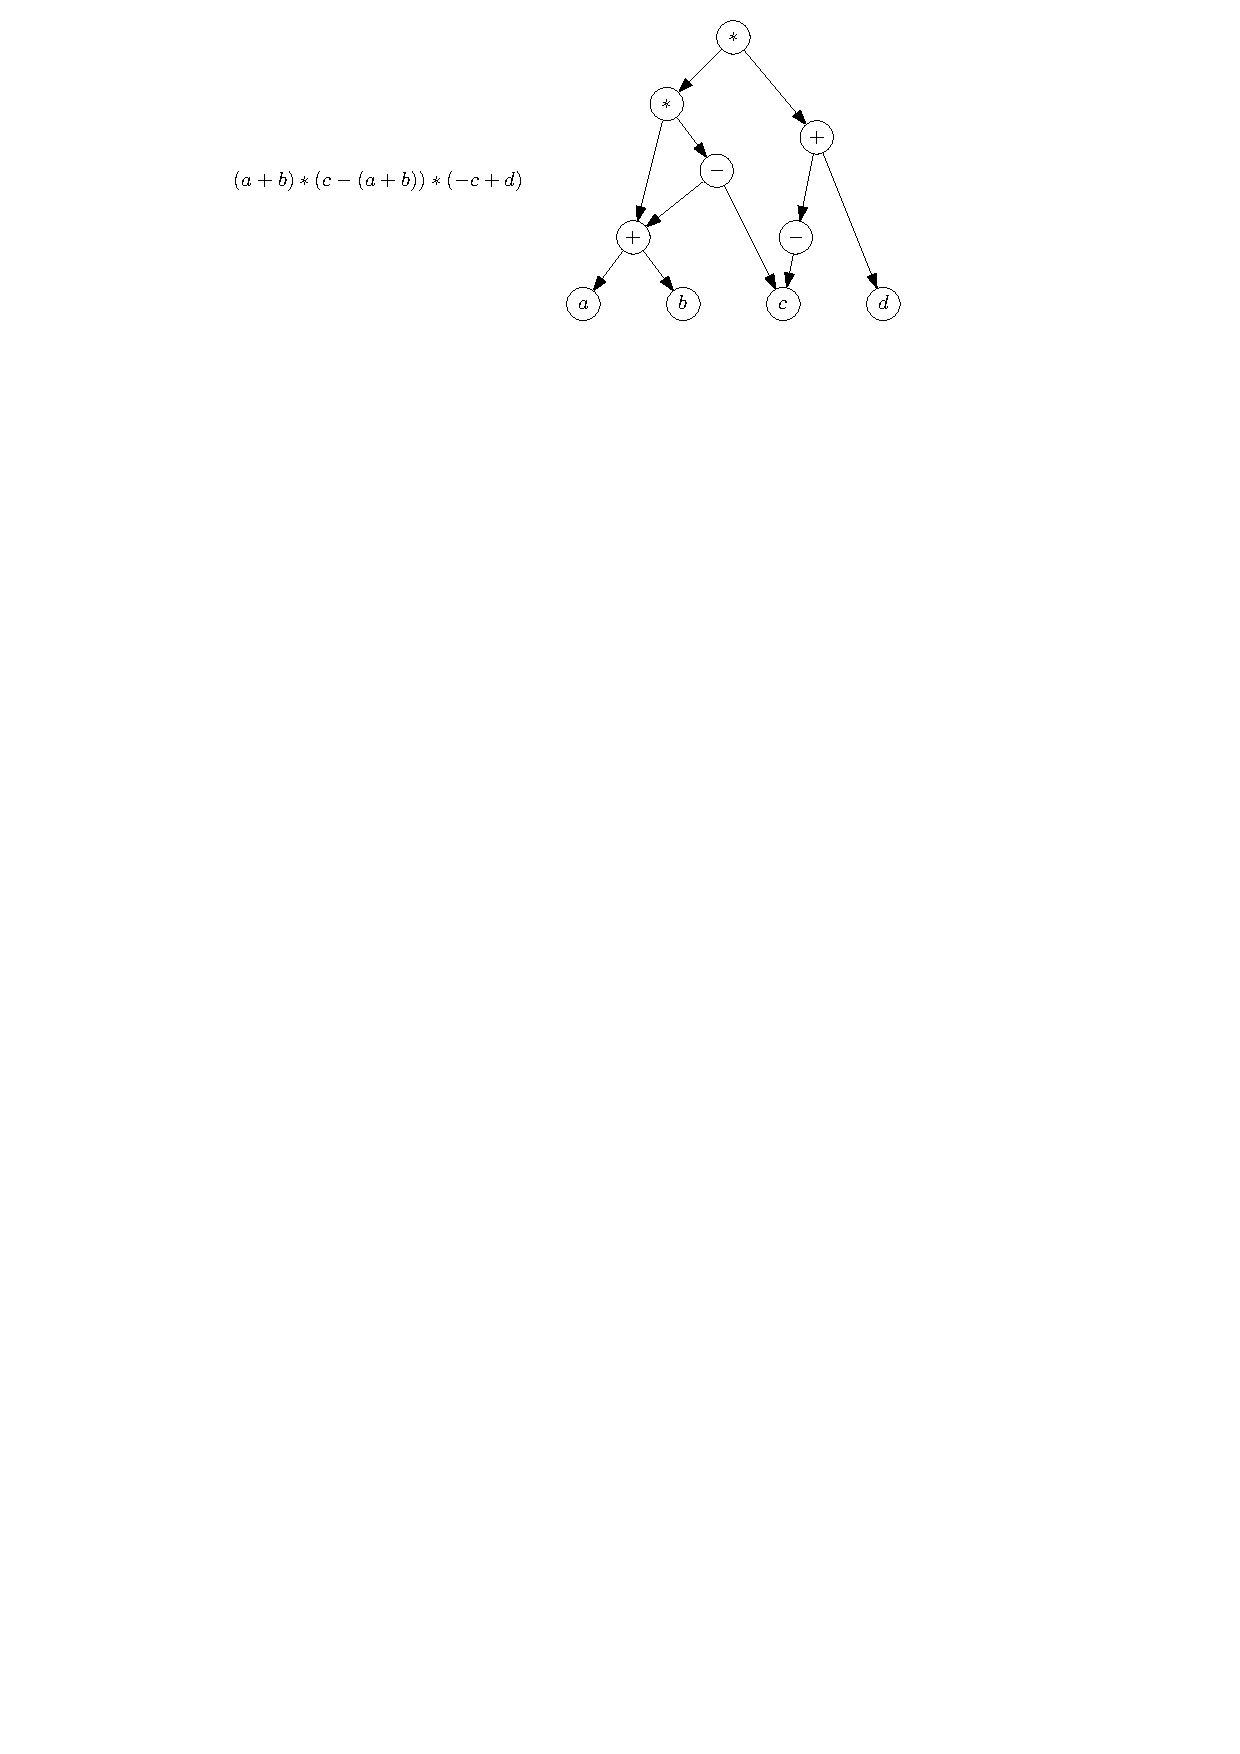
\includegraphics{precedence}
\end{Boxample}

Respecting all precedences/dependencies is equivalent to drawing the digraph 
with all nodes in a straight line and the arcs all pointing the same direction. 
The order of calculation starts at one end of the line and proceeds to the other.

\section{Topological sort}
\begin{Definition}
Let $G$ be a digraph. A \defnfont{topological sort} of $G$ is a linear
ordering of all its vertices such that if $G$ contains an arc $(u,v)$,
then $u$ appears before $v$ in the ordering. 
It is also known as a \defnfont{topological order} or \defnfont{linear order}.
\end{Definition}

For our arithmetic expression example above, a linear
order of the sub-expression digraph gives us an order (actually the reverse
of the order) where we can safely evaluate the expression.

\begin{Boxample}[1]
A graph with all possible topological orders and drawn with topological order $0, 1, 2, 3, 4$.  
Draw the graph for the topological order $0, 2, 1, 4, 3$. 
\begin{center}
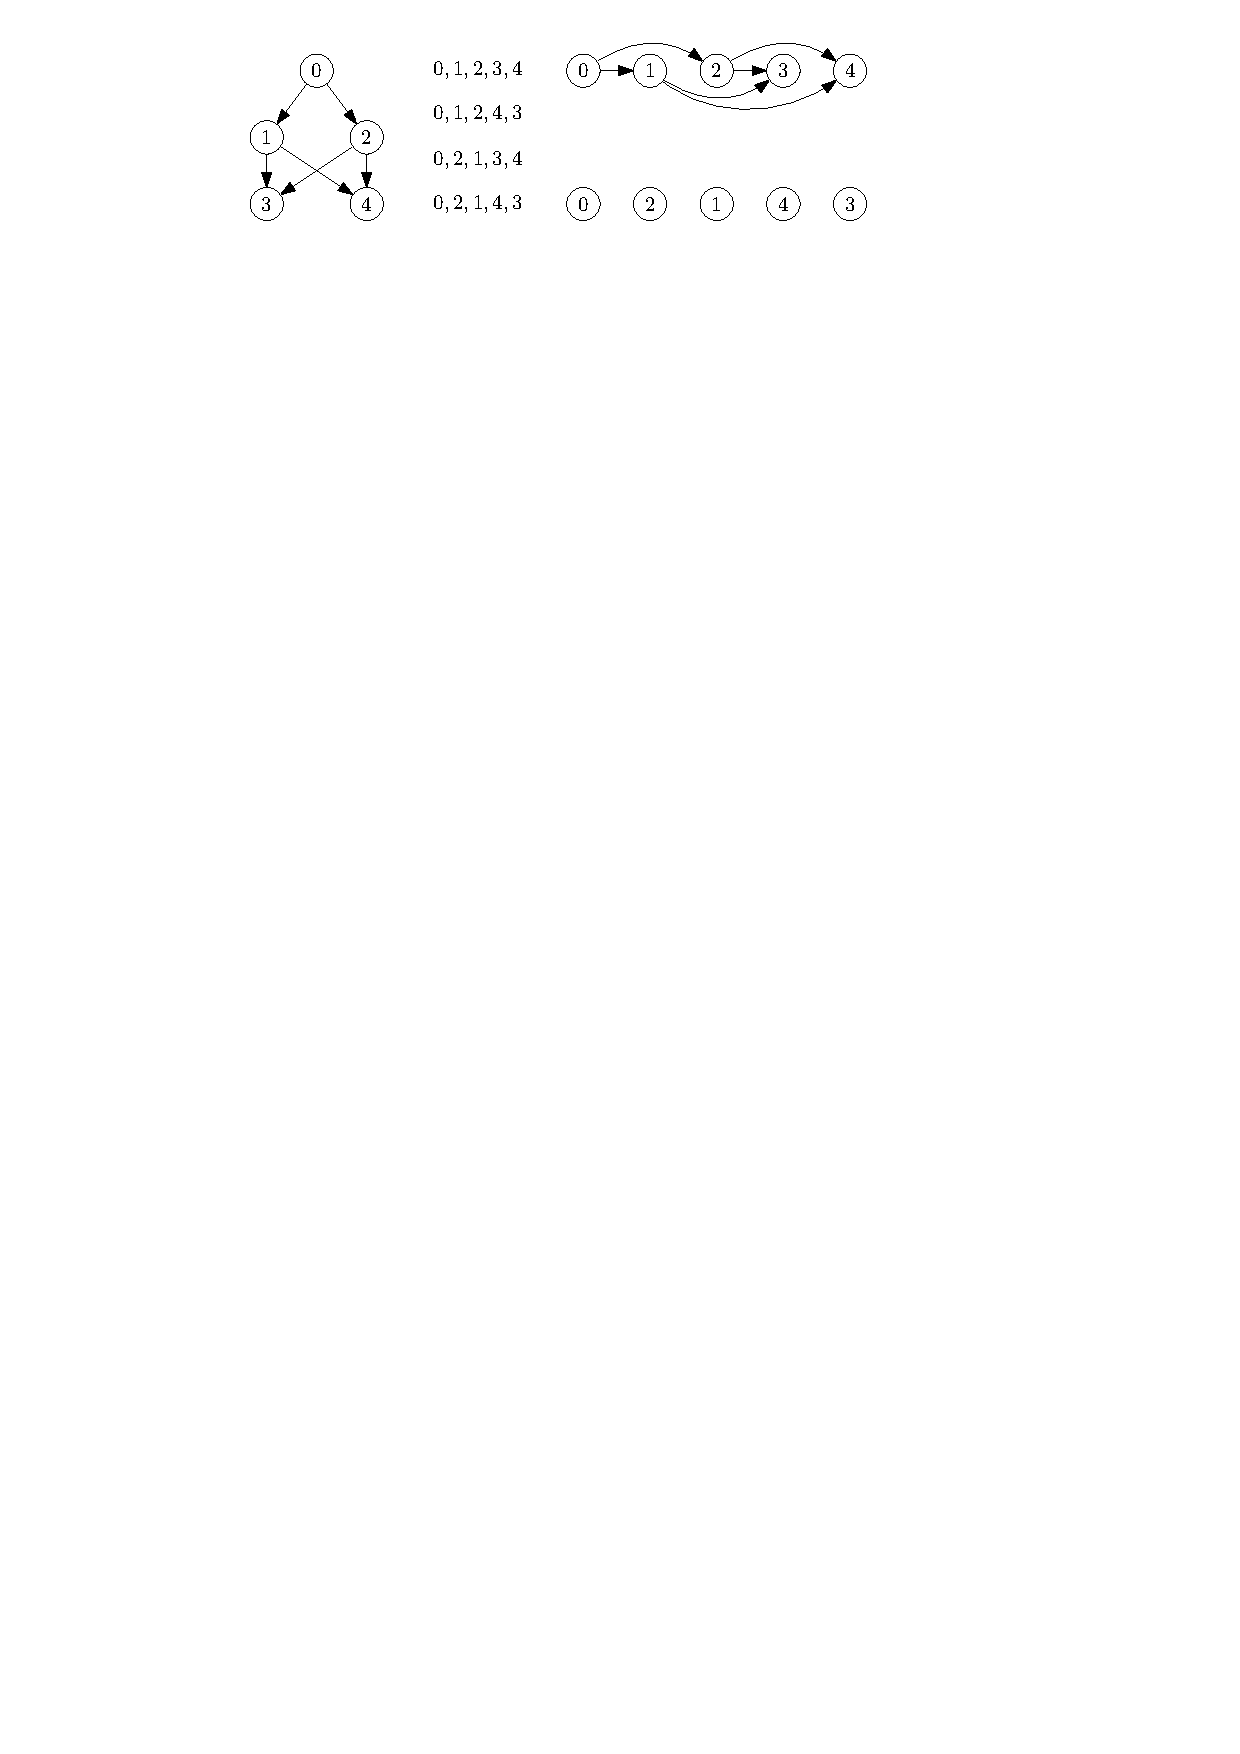
\includegraphics{topologicalOrder1}
\end{center}
Find a topological order of the following graph and draw it.
\begin{center}
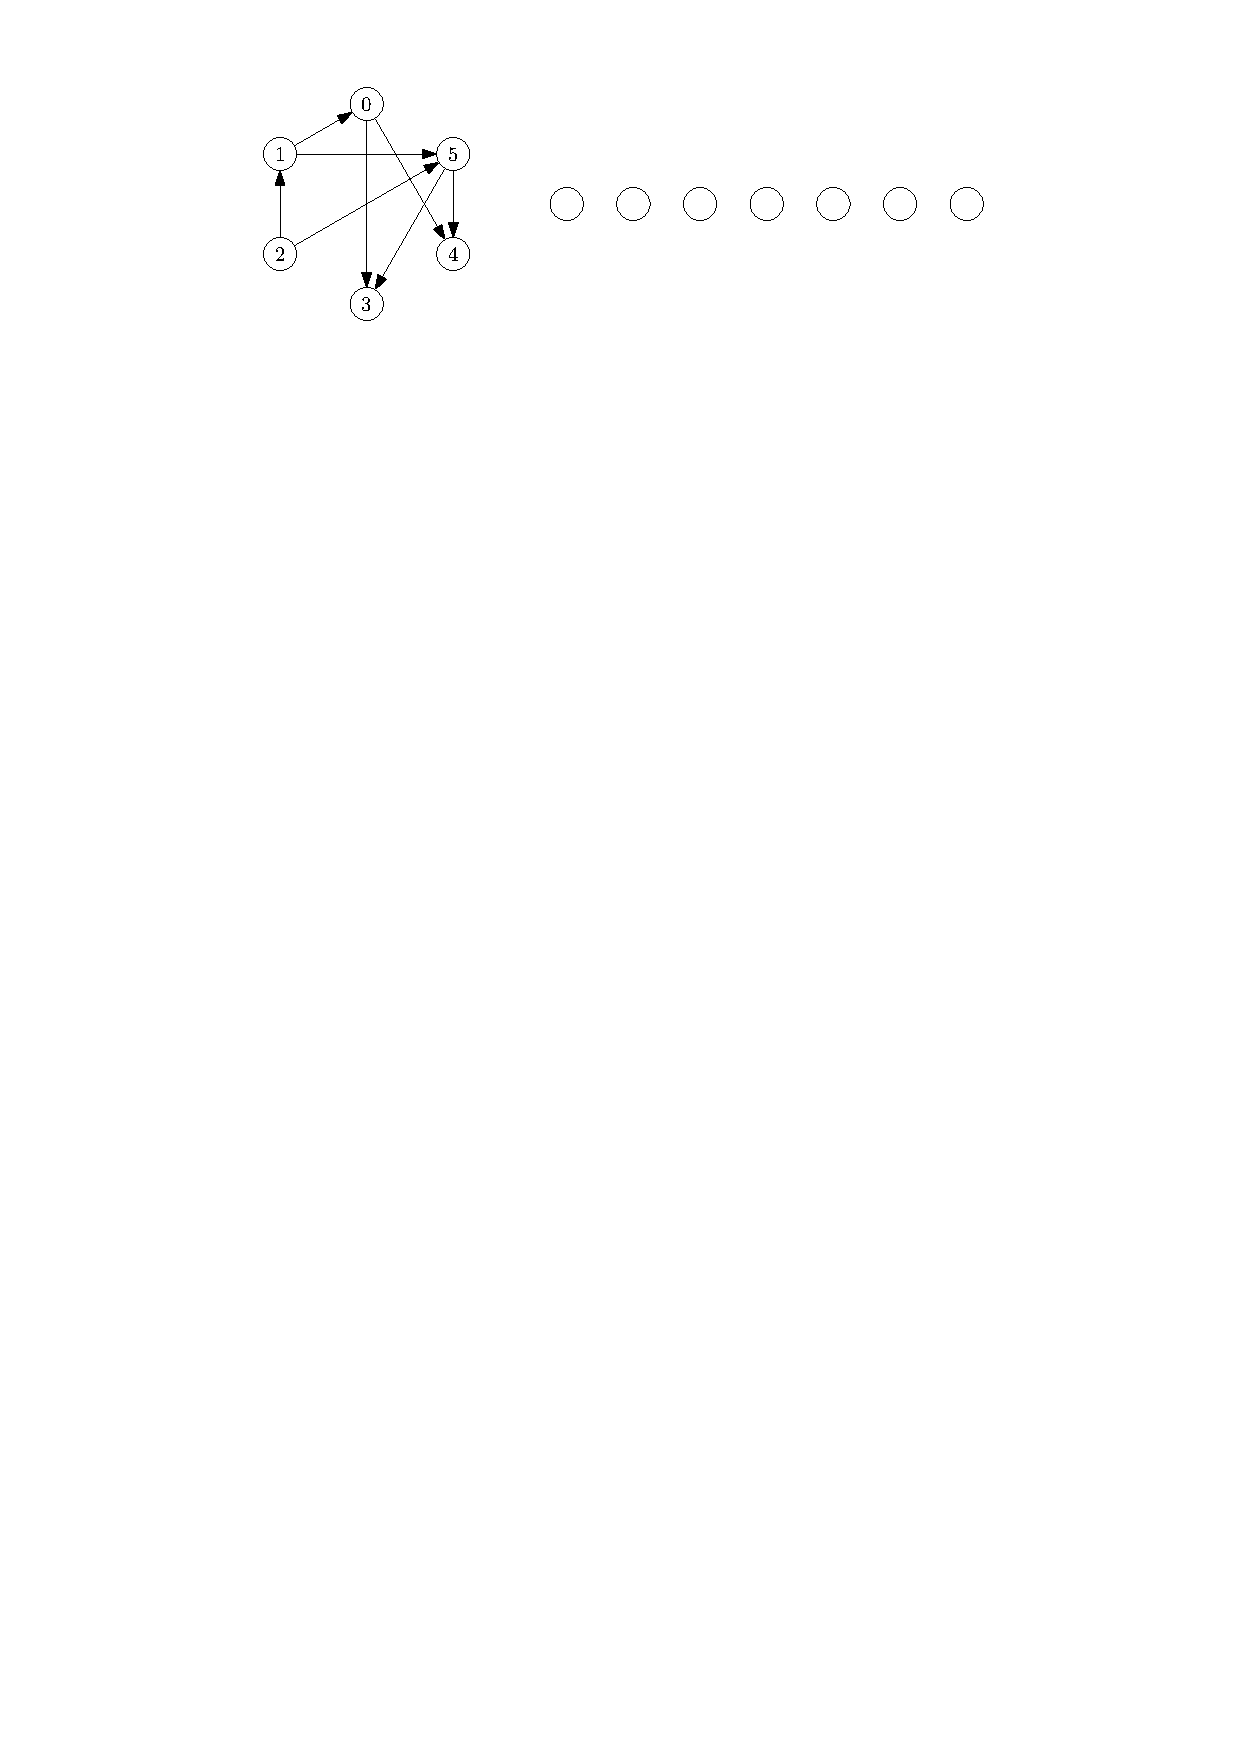
\includegraphics{topologicalOrder2}
\end{center}
Topological orders are not unique. List all possible topological orders of the following graph.
\begin{center}
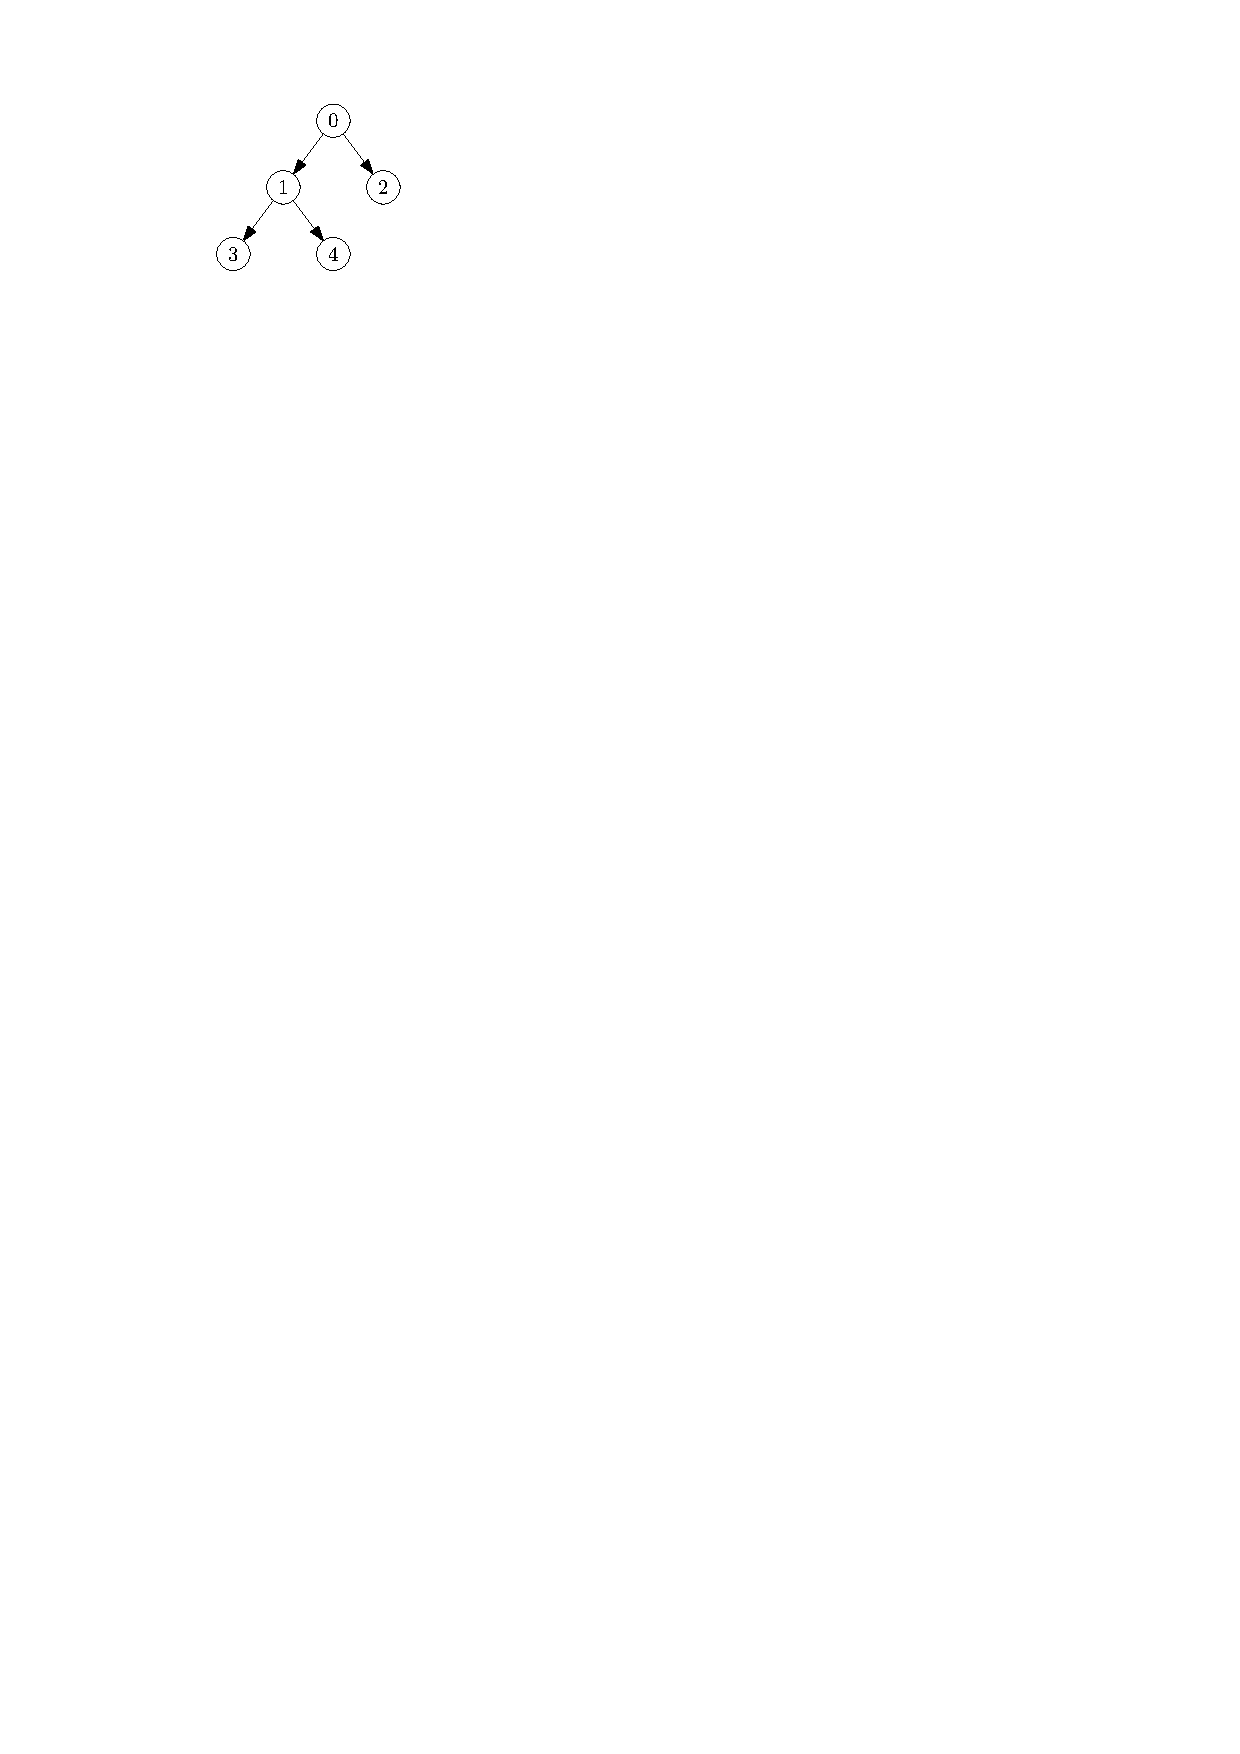
\includegraphics{topologicalOrder3}
\end{center}
\end{Boxample}

Clearly if the digraph contains a cycle, it is not possible to find
such a linear ordering. This corresponds to inconsistencies in the
precedences given, and no scheduling of the tasks is possible.

\begin{Definition}
A digraph without cycles is commonly called a \defnfont{DAG}, an
abbreviation for \textbf{d}irected \textbf{a}cyclic \textbf{g}raph.  
\end{Definition}

\begin{Theorem} \label{thm:topDAG}
A digraph has a topological order if and only if it is a DAG.
\end{Theorem}

\begin{Boxample}[8]
It is clear that if a digraph has a topological order it has no cycles, so it a DAG. 
Show that a DAG always has a topological order by first showing that every DAG has a source
and that by removing the source and any out-arcs from the source you still have a DAG. 
Show that the order in which nodes are removed gives a topological order.
\end{Boxample}

This theorem and proof then gives an algorithm \defnfont{zero-indegree sorting}
for topologically sorting a DAG. 
If we apply zero-indegree sorting to a digraph that is not a DAG, 
eventually it will stop because no source node can be found at some point.

\begin{Boxample}[3]
What is the running time of a naive implementation of zero-indgree sorting? Could this be improved upon?
\end{Boxample}

\section{Finding cycles and topological sorting using DFS}
DFS can be used to determine whether or not a digraph is a DAG and, if it is, find a topological sort.
\begin{itemize}
  \item Run DFS on $G$.
  \item If $G$ contains a cycle, the traversal will eventually reach a node that points to one that has been seen before. 
  In other words, we will detect a back arc. 
  \item If the traversal finds no back arcs, $G$ is a DAG 
  and the listing nodes in reverse order of DFS $\done$ times is a topological sort of $G$.
\end{itemize}

\begin{Theorem} \label{thm:findDAG}
Suppose that DFS is run on a digraph $G$. Then $G$ is acyclic if and only if there are no back arcs.
\end{Theorem}
%\begin{proof}
%Suppose that we run DFS on $G$. Note that if there is a
%back arc $(v, u)$, then $u$ and $v$ belong to the same tree $T$, with
%root $s$ say. Then there is a path from $s$ to $u$, and there is a path
%from $u$ to $v$ by definition of back arc. Adding the arc $(v, u)$ gives
%a cycle. 
%
%Conversely, if there is a cycle $v_0\, v_1\, \dots \, v_n\, v_0$, we may
%suppose without loss of generality that $v_0$ is the first node of the
%cycle  visited by the DFS algorithm. We claim that $(v_n, v_0)$ is a
%back arc. To see why this is true, first note that during the DFS $v_0$ is 
%linked to $v_n$ via a path of unvisited nodes (possibly of length shorter 
%than $n$).  We have $v_n$ as a descendant of $v_0$ in the DFS tree and
%a back arc $(v_n, v_0)$.
%\end{proof}

\begin{Theorem}
Let $G$ be a DAG. Then listing the nodes in reverse order of DFS
finishing times yields a topological order of $G$.
\end{Theorem}
\begin{proof} 
Consider any arc $(u,v) \in E(G)$. 
Since $G$ is a DAG, the arc is not a back arc by \cref{thm:findDAG}. 
In the other three cases, \cref{ex:DFS-arc-class} shows that $\done[u] > \done[v]$,
which means $u$ comes before $v$ in the alleged topological order.
\end{proof}

Note that printing the nodes in order of finishing time gives a topological order of the reverse digraph $G_r$.

%\begin{Boxample}[2] \label{ex:DAG-vs-tree}
%Give an example of a DAG whose underlying graph contains a cycle. Make
%your example as small as possible.
%\end{Boxample}

%\begin{Boxample} \label{ex:sillytopsort}
%Show that the following method for topologically sorting a DAG does not work in 
%general: print the nodes in order of visiting time.
%\end{Boxample}

%\begin{Boxample} \label{ex:profP}
%Professor P has the following information taped to his mirror, to help
%him to get dressed in the morning.
%
%Socks before shoes; underwear before trousers; trousers before belt;
%trousers before shoes; shirt before glasses; shirt before tie; tie
%before jacket; shirt before hat; shirt before belt.
%
%Find an acceptable order of dressing for Professor P.
%\end{Boxample}

%\begin{Boxample} \label{ex:forest}
%Let $G$ be a graph. There is an easy way to show that $G$ is acyclic.
%It is not hard to show (see Section~\ref{sec:app:trees}) that a graph $G$ is 
%acyclic if and only if $G$ is a forest, that is, a union of (free) trees.
%
%Give a simple way to check whether a graph $G$ is acyclic. Does the method 
%for finding a DAG given above work for acyclic graphs also?
%\end{Boxample}

\section{The girth of a graph} \label{sec:girth}
The length of the smallest cycle in a graph is an important quantity. 
For example, in a communication network, short cycles are often something to be
avoided because they can slow down message propagation.

\begin{Definition}
The \defnfont{girth} of the graph is the length of the shortest cycle. If the graph has no cycles then the
girth is undefined but may be viewed as $+\infty$. 

For a digraph we use the term girth for its underlying graph and the (maybe non-standard) term \defnfont{directed girth} for
the length of the smallest directed cycle.
\end{Definition}

\begin{Boxample}[0]
What are the girth and the directed girth of the following digraph?
\begin{center}
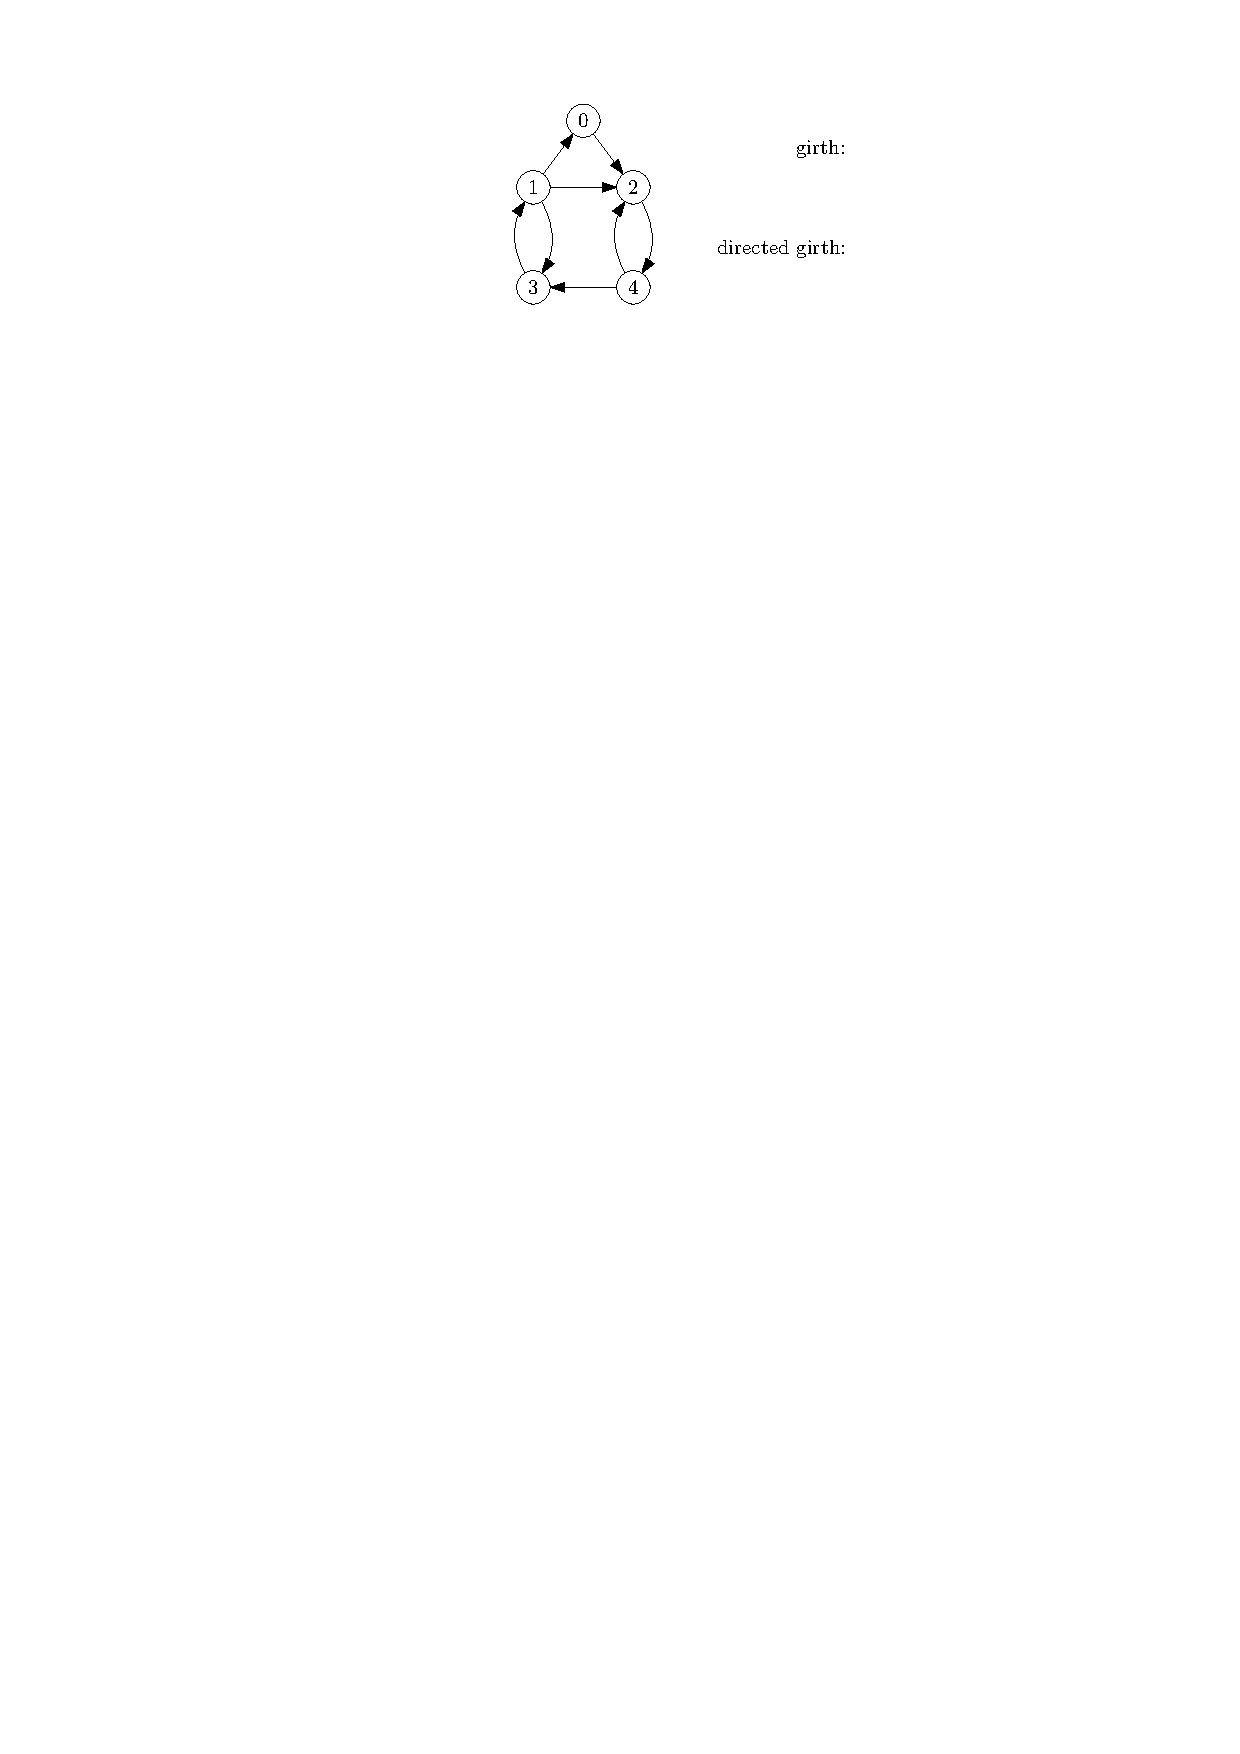
\includegraphics{girthEx}
\end{center}
\end{Boxample}




\chapter{Finding girth, connectivity, components, strong components} %-----------------------

\section{Finding the girth of a graph with BFS}
How to compute the girth of a graph? Here is an algorithm for finding
the length of a shortest cycle containing a given vertex $v$ in a graph $G$. 
\begin{itemize}
  \item Perform \texttt{BFSvisit}. 
  \item If we meet a grey neighbour 
  (that is, we are exploring edge $\{x, y\}$ from $x$ and we find that $y$ is already grey), 
  continue only to the end of the current level and then stop.
  \item For each edge $\set{x, y}$ as above on this level, 
  if $v$ is the lowest common ancestor of $x$ and $y$ in the BFS tree, then there is a cycle
  containing $x, y, v$ of length $l=d(x) + d(y) + 1$. 
  \item Report the minimum value of $l$ obtained along the current level.
\end{itemize}

\begin{Boxample}[8] \label{ex:BFS-cycle} 
Prove above algorithm is correct.
{\color{red} TODO: need to proide some pointers here on how to prove}
%\end{Theorem}
%\begin{proof}
%Suppose that we arrive at vertex $x$, $d(x) = k$, and we have just
%encountered a grey neighbour $y$. Then $d[y] = d[x] + 1$ or $d[y] = d[x]$
%(note that $d[x] = d[y] + 1$ is ruled out because then $x$ would be a
%child of $y$ and $y$ would be black). This means that there is definitely
%a cycle containing $x, y$ and $z$, where $z$ is the lowest common ancestor
%of $x$ and $y$ in the BFS tree. Note that $z\neq x, z\neq y$ since neither
%$x$ nor $y$ is an ancestor of the other. The cycle consists of the tree
%edges from $z$ to $x$, the cross edge $\set{x,y}$ and the tree edges
%from $z$ to $y$. The length of the cycle is $l=d[x] + d[y] - 2 d[z] + 1$.
%
%Conversely, let $C$ be any cycle and let $z$ be the first vertex of
%the cycle reached by the search. Let $x$ and $y$ be two vertices in $C$
%whose distance  from $z$ is greatest, with $d[x] \leq d[y]$. Then the
%lowest common ancestor of  $x$ and $y$ is exactly $z$, and the cycle
%found in the first paragraph is exactly $C$.
%
%The vertex $v$ belongs to the cycle $C$ if and only if $v = z$. The
%length of the cycle is $2k+1$ if $d[x] = d[y]$ and $2k+2$ if $d[y] =
%d[x] - 1$. The minimum length of any cycle containing $v$ found after
%this is $2(k+1) + 1 = 2k+3$, so no better cycle can be found after the
%current level $k$ is explored.
\end{Boxample}

To compute the girth of a graph, we can simply run the above algorithm
from each vertex in turn, and take the minimum cycle length achieved.

\begin{Boxample}
An easy-to-implement DFS idea may not work properly. 
Consider the DFS tree originating from vertex $0$ of the graph below. 
Which is the smallest cycle it finds with the back edges? Which smaller cycle does it miss?
\begin{center}
  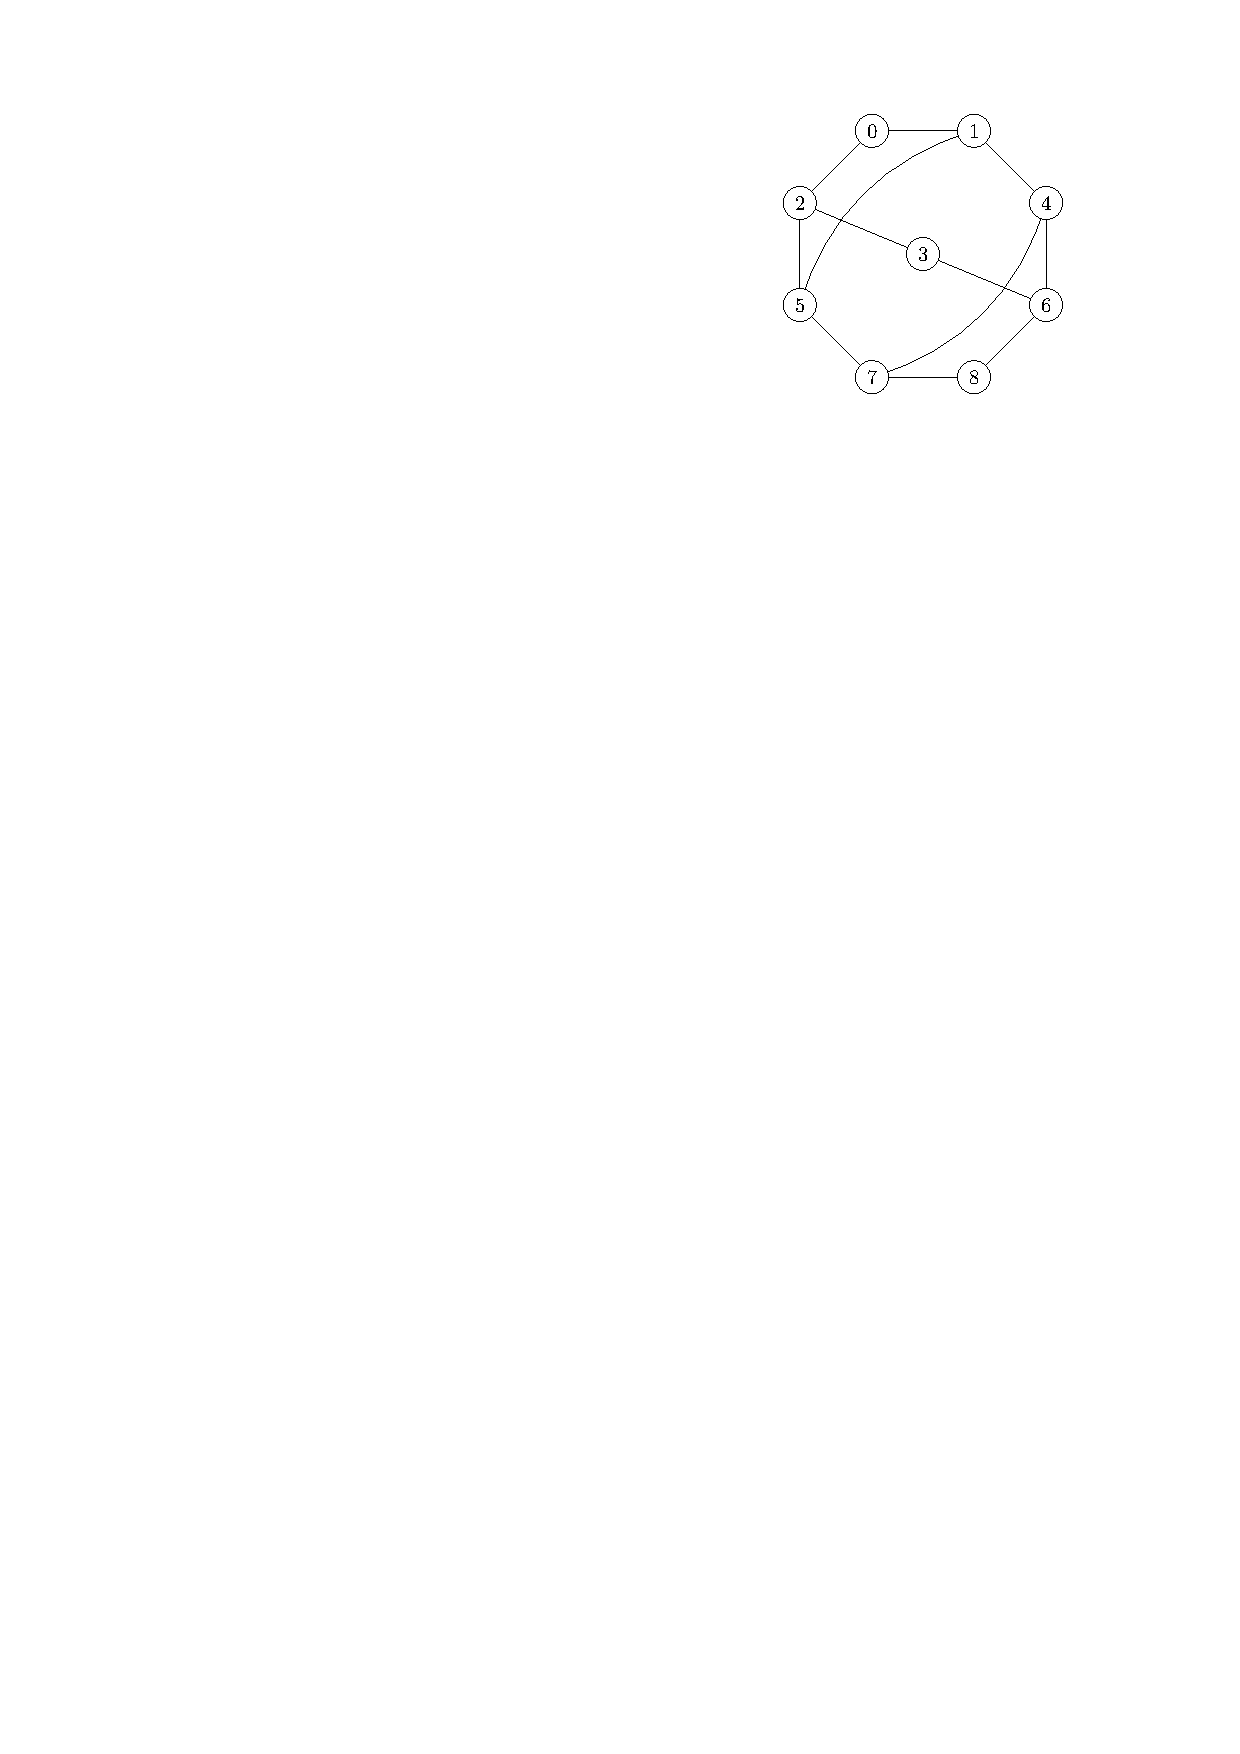
\includegraphics{girthEx2}
\end{center}
\end{Boxample}

% \begin{Boxmaple} \label{ex:shortest-cycle-thm}
% Give an example to show that in the shortest cycle algorithm, if we
% do not continue to the end of the level, but terminate when the first
% cycle is found, we may find a cycle whose length is one more than the
% shortest possible.
% \end{Boxmaple}
% TODO: include this?

\section{Finding the directed girth of a digraph with DFS}
{\color{red}TODO section}


\section{Connectivity in graphs}
%For many purposes it is useful to know whether a digraph is ``all in one
%piece", and if not, to decompose it into pieces. We now formalize these
%notions. The situation for graphs is easier than that for digraphs.

For many purposes it is useful to know whether a digraph is ``all in one
piece", and if not, to decompose it into pieces.


\begin{Definition} 
A graph is \defnfont{connected} if for each pair of 
vertices $u, v \in V(G)$, there is a path between them.
\end{Definition}

\begin{Theorem} \label{thm:components}
Let $G$ be a graph. Then $G$ can be uniquely written as a union of
subgraphs $G_i$ with the following properties:
\begin{itemize}
  \item each $G_i$ is connected,
  \item if $i \neq j$, there are no edges from any vertices in $G_i$ 
  to any vertices in $G_j$.
\end{itemize}
\end{Theorem}
%\begin{proof}
%Consider the relation $\sim$ defined on $V(G)$, given by $u\sim v$ if
%and only if there is a path joining $u$ and $v$ (in other words, $u$ and
%$v$ are each reachable from the other). Then $\sim$ is an equivalence
%relation and so induces a partition of $V(G)$ into disjoint subsets. The
%subgraphs $G_i$ induced by these subsets have no edges joining them by
%definition of $\sim$, and each is connected by definition of $\sim$.
%\end{proof}

The subgraphs $G_i$ above are called the \defnfont{connected components} of the graph $G$. 
Clearly, a graph is connected if and only if it has exactly one connected component.

\begin{Boxample} \label{eg:components}
The graph obtained by deleting two edges from a triangle has 2 connected components.
\end{Boxample}

We can determine the connected components of a graph easily by using a
traversal algorithm. The following obvious theorem explains why.

\begin{Theorem} \label{thm:trav-comps}
Let $G$ be a graph and suppose that DFS or BFS is run on $G$. Then the
connected components of $G$ are precisely the subgraphs spanned by the
trees in the search forest. 
\end{Theorem}

So to find the components of a graph $G$:
\begin{itemize}
\item Run BFS or DFS on $G$ and count of the number of times we choose a root -- this is the number of components.
\item Store or print the vertices and edges in each component as we explore them.
\item This is a linear time algorithm, $O(m+n)$.
\end{itemize}

\section{Connectivity in digraphs}
The intuition of a digraph being ``all in one piece" is not as useful as it was for graphs. 

\begin{Boxample}[0]
This digraph appears to be ``all in one piece'' as its underlying graph is connected. 
But can you get from any node to any other node following the direction of the arcs?
\begin{center}
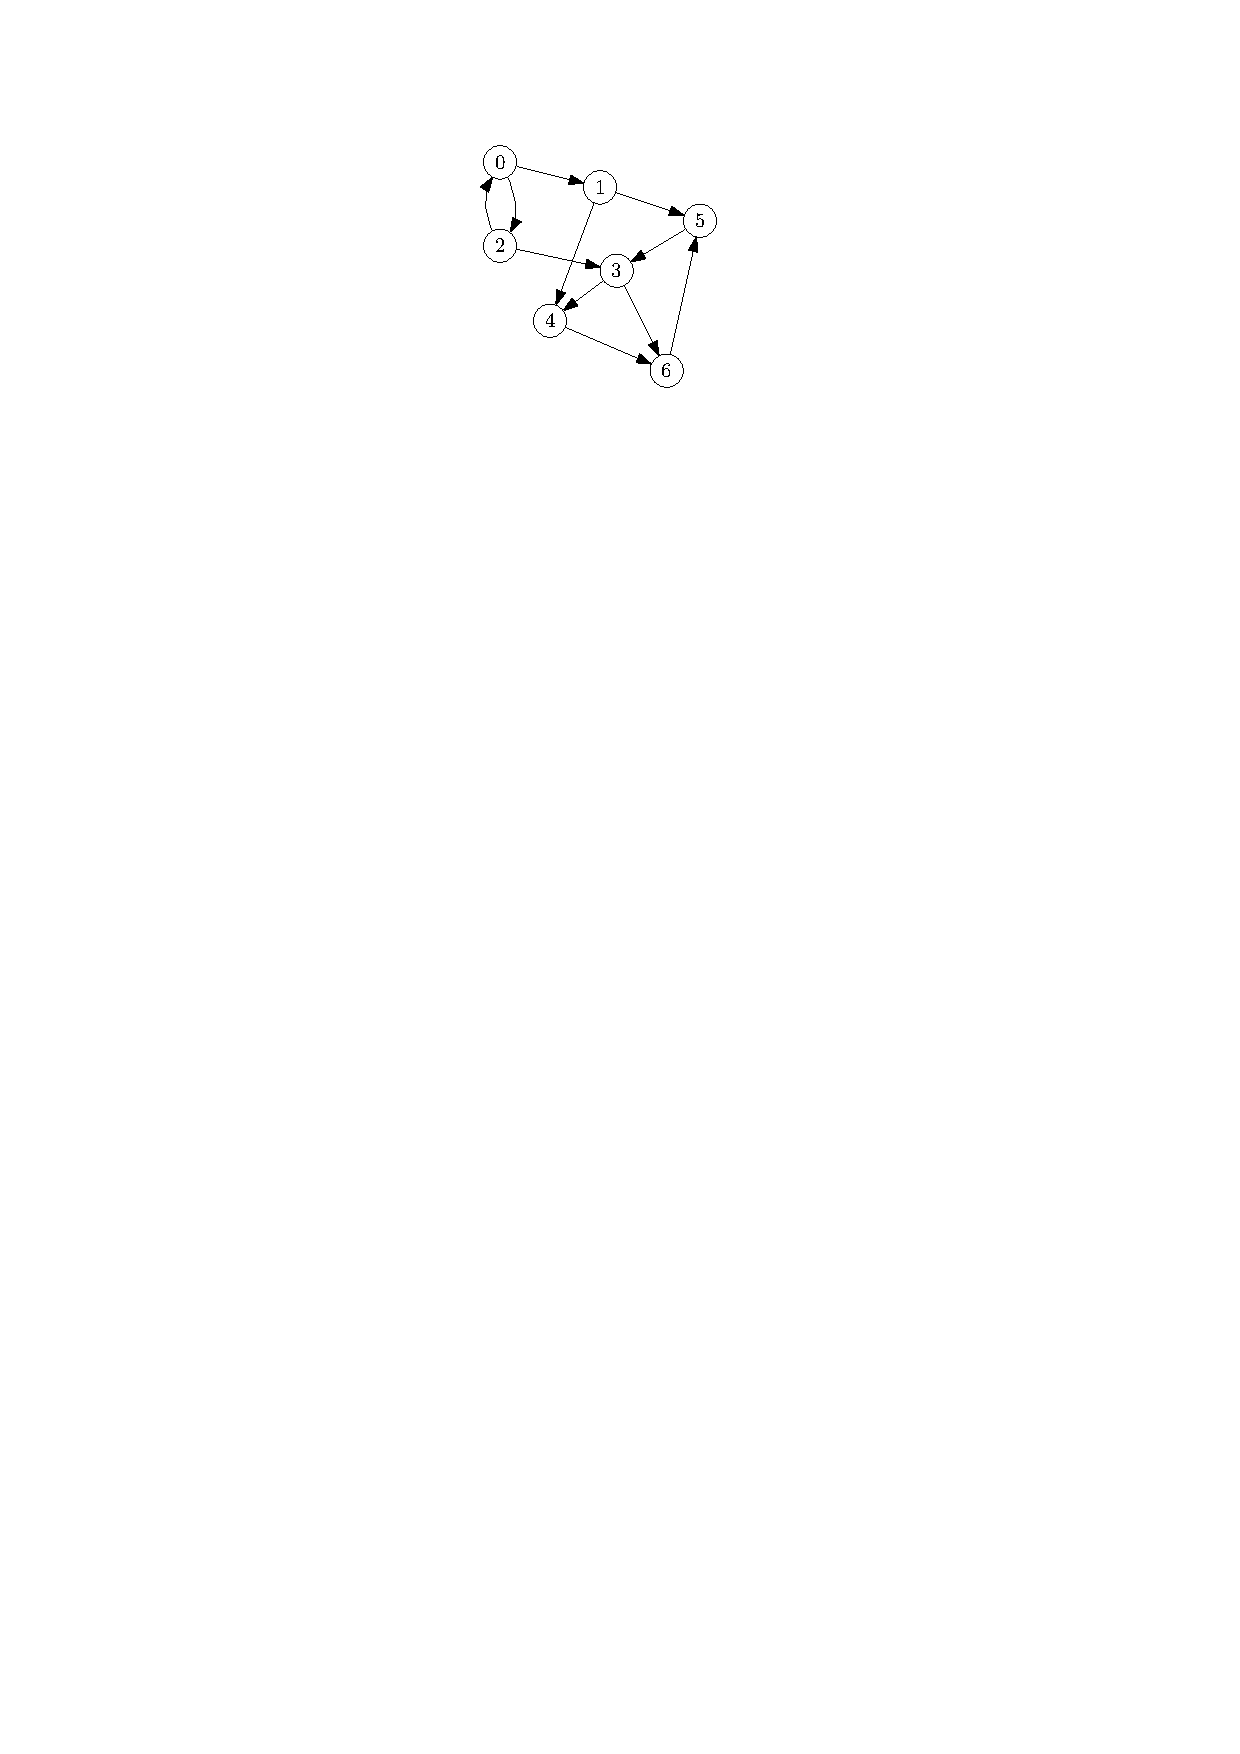
\includegraphics{connectedComponentDigraph}
\end{center}
\end{Boxample}

This example motivates the following definition.

\begin{Definition}
A digraph $G$ is \defnfont{strongly connected} if for each pair of nodes $u$, $v$ 
of $G$, there is a path in $G$ from $u$ to $v$ and from $v$ to $u$ (that is, $u$ and $v$ are reachable from one another).
\end{Definition}

\begin{Boxample}[4]
Show that a strongly connected digraph of order at least three contains at least one cycle.
% Note: Definition of cycle says cycle must contain at lesat three vertices, hence example with ``order at least two'' doesn't work.
\end{Boxample}

\begin{Definition} 
A \defnfont{strongly connected component}, $G_i$, of $G$ is a maximal sub-digraph of $G$ 
such that $G_i$ is strongly connected. 
All nodes of $G$ are in exactly one such $G_i$, so the partition into strongly connected components is unique.
\end{Definition}

%%\newpage
%\begin{Theorem}
%\label{thm:scc}
%Let $G=(V, E)$ be a digraph. Then $V$ can be uniquely written as a union of
%disjoint subsets $V_i$, with each corresponding induced subdigraph $G_i$ being
%a strongly connected component of $G$.
%\end{Theorem}
%
%\begin{proof} Consider the relation $\sim$ defined on $V$, given by
%$u\sim v$ if and only if there is a path joining $u$ and $v$ and a path
%joining $v$ and $u$ (in other words, $u$ and $v$ are each reachable
%from the other). Then $\sim$ is an equivalence relation and so induces
%a partition of $V$ into disjoint subsets.  By definition, each 
%subdigraph $G_i$ is strongly connected and of maximal order.
%\end{proof}

\begin{Boxample}[0]\label{eg:scc}
This digraph has three strongly connected components. Find and draw the two missing ones.\\

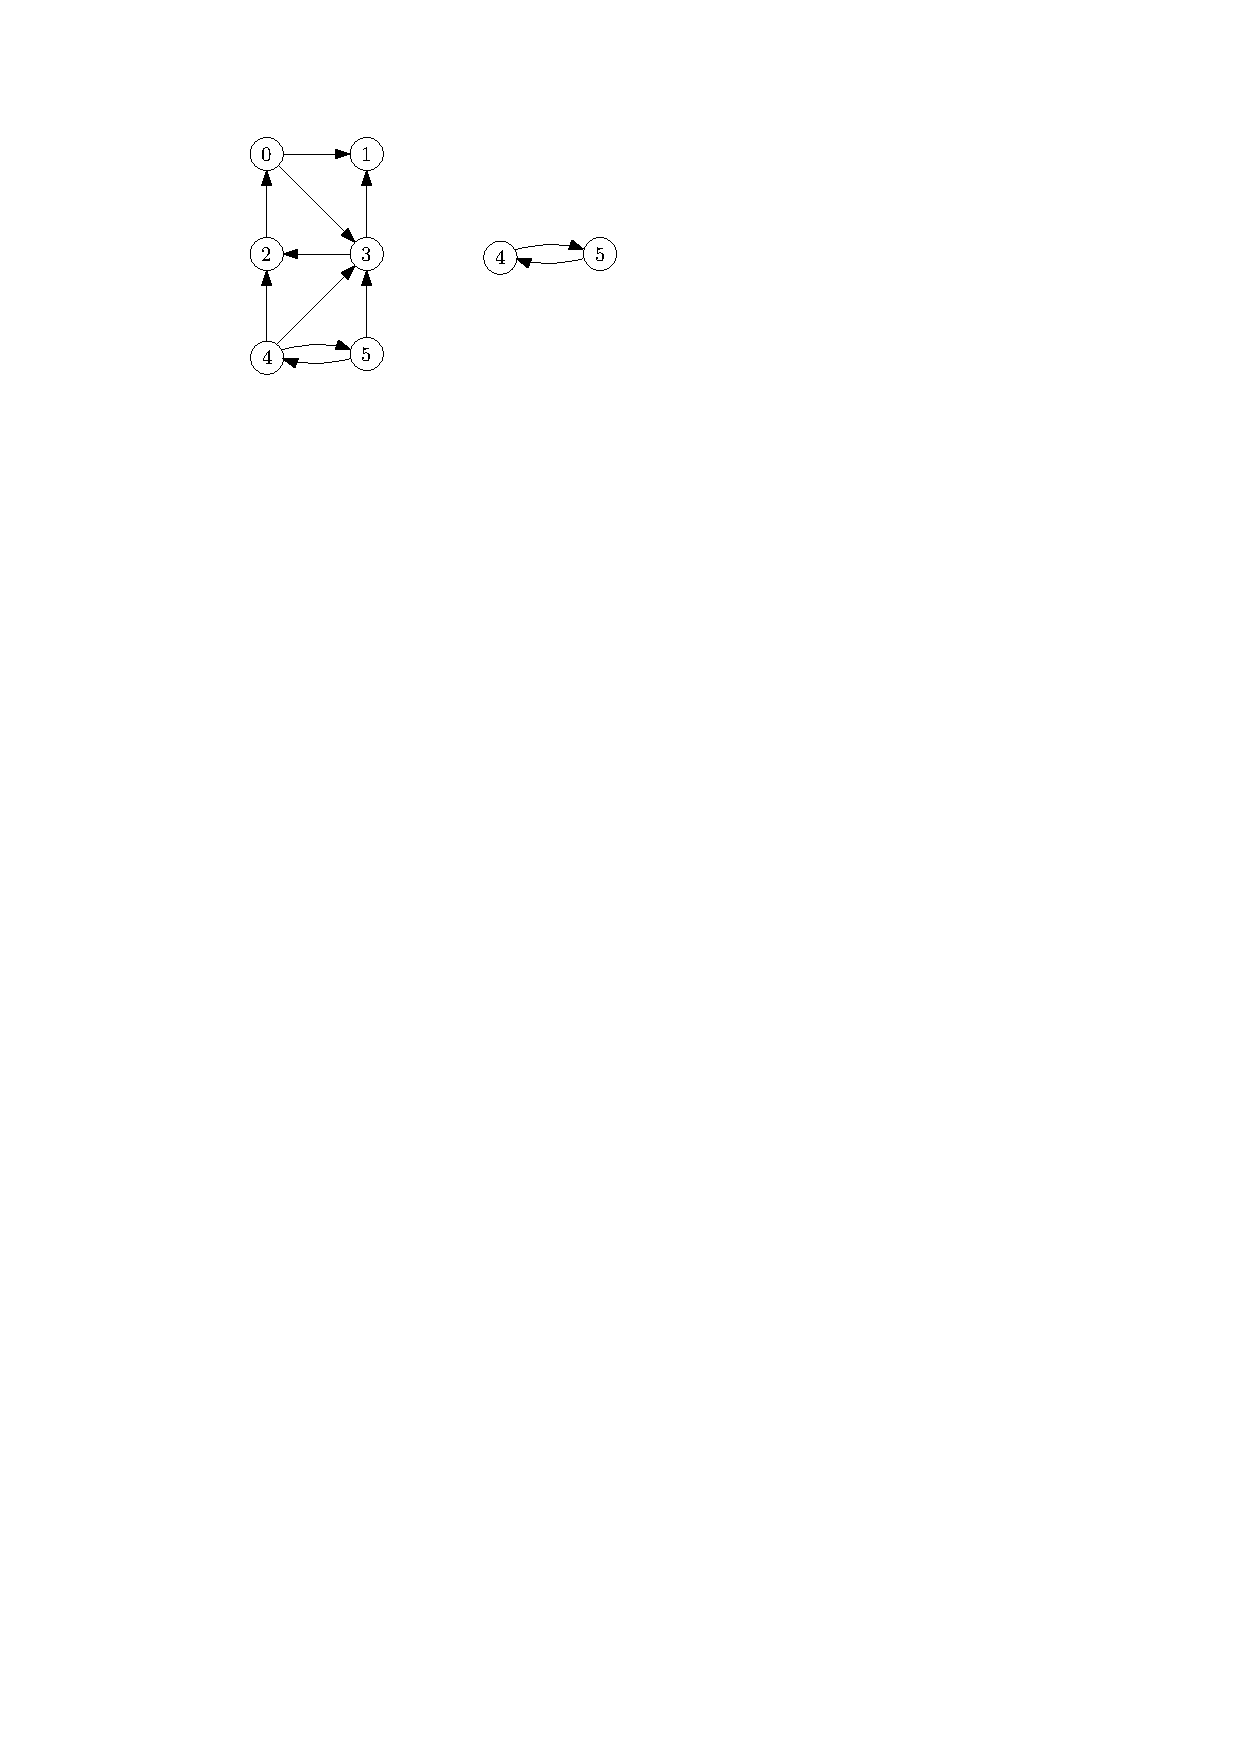
\includegraphics{SCCex}

Note that there are arcs of the digraph not included in the strongly connected components.
\end{Boxample}

\begin{Boxample}[4]
Find a counter-example to show that the method for finding connected components of graphs 
in \cref{thm:trav-comps} fails at finding strongly connected components of digraphs.
\end{Boxample}



%\subsection*{Exercises}
%
%\begin{Exercise}
%\label{ex:DFSfails}
%Give an example to show that a single use of DFS does not in general
%find the strongly connected components of a digraph.
%\end{Exercise}
%
%\begin{Exercise}
%\label{ex:dolinscc}
%Carry out the above  algorithm by hand on the digraph of
%\cref{eg:scc} and verify that the components given there are
%correct. Then run it again on the reverse digraph and verify that the
%answers are the same.
%\end{Exercise}


\chapter{Finding Strong components, bipartite graphs} %--------------------------------------------------

\section{Finding the strongly connected components}

%Note that if the underlying graph of $G$ is connected but $G$ is
%not strongly connected, then  there are strong components $C_1$ and
%$C_2$ such that it is possible to get from $C_1$ to $C_2$ but not
%from $C_2$ to $C_1$. If $C_1$ and $C_2$ are different strong
%components, then any arcs between them must either all point from
%$C_1$ to $C_2$ or from $C_2$ to $C_1$.  Suppose that we imagine
%each strong component shrunk to a single node (so we ignore the
%internal structure of each component, but keep the arcs between
%components). Then in the digraph resulting, if $v\neq w$ and we can
%get from $v$ to $w$ then we cannot get from $w$ to $v$. In other
%words, no pair of nodes can belong to a cycle, and hence the digraph
%is acyclic. See \cref{fig:sccdecomp}. Note that the converse
%is also true: if we have an acyclic digraph $G$ and replace each
%node by a strongly connected digraph, the strongly connected
%components of the resulting digraph are exactly those digraphs that
%we inserted.

%Note the similarity between this and the search forest decomposition
%in \cref{fig:travdecomp}. In that case, if we shrink each
%search tree to a point, the resulting digraph is also acyclic.


We can determine if $G$ is strongly connected or not (i.e., has a single strongly connected component) 
by running \texttt{BFSvisit} or \texttt{DFSvisit} originating from each node in turn. 
If it is strongly connected, all trees produced will span $G$. 
The running time of such an algorithm is $\Theta(n^2+nm)$.

{\color{red} TODO: compress and clarify this argument. OK to omit formal proof if decent intuition is given}

We can do better by using DFS more cleverly. 

Consider the reverse $G_r$. The strong components of $G_r$ are the
same as those of $G$. Shrinking each strong component to a point,
we obtain  acyclic digraphs $H$ and $H_r$. Consider a sink $S_1$ in
$H_r$. If we run DFS on $G_r$ starting  in the strong component
$S_1$, we will reach every node in that component \boldfont{and no
other nodes of $G_r$}. The DFS tree will exactly span $S_1$. Now
choose the next root to lie in the strong component $S_2$ node of
$H_r$ whose only possible out-neighbour is $S_1$ (this is possible
by the same reasoning used for zero-indegree sort, except here we
deal with outdegree). The DFS will visit all of $S_2$ and no other
nodes of $G_r$ because all other possible nodes have already been
visited. Proceed in this way until we have visited all strong
components.

We have shown that if we can choose the roots correctly, then we can
find all strong components. Now of course we do not know these components
\boldfont{a priori}, so how do we identify the roots to choose?

Whenever there is a choice for the root of a new search tree, it must
correspond to a new node of the DAG $H_r$. We want at least a reverse
topological order of $H_r$. This is simply a topological order for
$H$. Note that in the case where $H=G$ (each strong component has just
one point), then $G$ is a DAG. The method above will work if and only
if we choose the roots so that each tree in the DFS for $G_r$ has only
one point. We just need a topological order for $G$, so run DFS on $G$
and print the nodes in reverse order of finishing time. Then choose the
roots for the DFS on $G_r$ in the printed order.

It therefore seems reasonable to begin with a DFS of $G$. Furthermore,
an obvious choice is: in the DFS of $G_r$, \boldfont{choose each new root
from among white nodes that finished latest in $F$}.

Then each DFS tree in the search of $G_r$ definitely contains the strong
component $S$ of the root $r$. To see this, note that no node in that
strong component could have been visited before in $G_r$, otherwise $r$
would have already been visited. By \cref{thm:white-path}, every
node in the strong component of $r$ is a descendant of $r$.

The only thing that could go wrong is that a search tree in $G_r$
might contain more than one strong component. This cannot happen,
as we now prove.

\begin{Theorem} \label{thm:scc-alg} 
If the following rule for choosing roots is used in the algorithm
described above, then each tree in the second search forest spans a
strong component of $G$, and all strong components arise this way.

Rule: use the white node whose finishing time in $F$ was largest.
\end{Theorem}

%\begin{proof}
%Suppose that a search tree in $G_r$ does  contain more than one strong
%component. Let $S_1$ be the first strong component seen in $G_r$ and let
%$S_2$ be another, and let the roots be $r, s$ respectively. Note that by
%the rule for choosing nodes $r$ was the first node of $S_1$ seen in $F$
%(by Theorem~\ref{thm:white-path}, every node of $S_1$ is a descendant
%of the first one seen, which therefore has latest finishing time). The
%analogous statement holds for $s$ and $S_2$.
%
%By the rule for choosing roots, we have $\done[r] > \done[s]$ in $F$. We
%cannot have $\seen[s] > \seen[r]$ in $F$, for then $s$ would be a descendant
%of $r$ in $F$ and in $G_r$, so they would belong to the same strong
%component. Thus $\seen[r] > \seen[s]$ in $F$. Hence $S_2$ was explored
%in $F$ before $r$ (and hence any node of $S_1$) was seen. But then $r$
%would have been reachable from $s$ in $G$ via a path of white nodes,
%so Theorem~\ref{thm:white-path} shows that $r$ and $s$ are in the same
%strong component, another contradiction.
%\end{proof} 

The above algorithm runs in linear time with adjacency lists, since each
DFS and the creation of the reverse digraph take linear time. We only
need to remember  while performing the first DFS to store the nodes in
an array in order of finishing time. 

\section{Bipartite graphs}

Many graphs in applications have two different types of nodes, and no
relations between nodes of the same type (this is a model of sexually
reproducing organisms, for example).

\begin{Definition}
A graph $G$ is \defnfont{bipartite} if $V(G)$  can be partitioned into
two nonempty disjoint subsets $V_0, V_1$ such that each edge of $G$
has one endpoint in $V_0$ and one in $V_1$.
\end{Definition}

\begin{Boxample} \label{ex:bipartite}
This graph is bipartite.  
The isolated vertex could be placed on either side.
\begin{center}
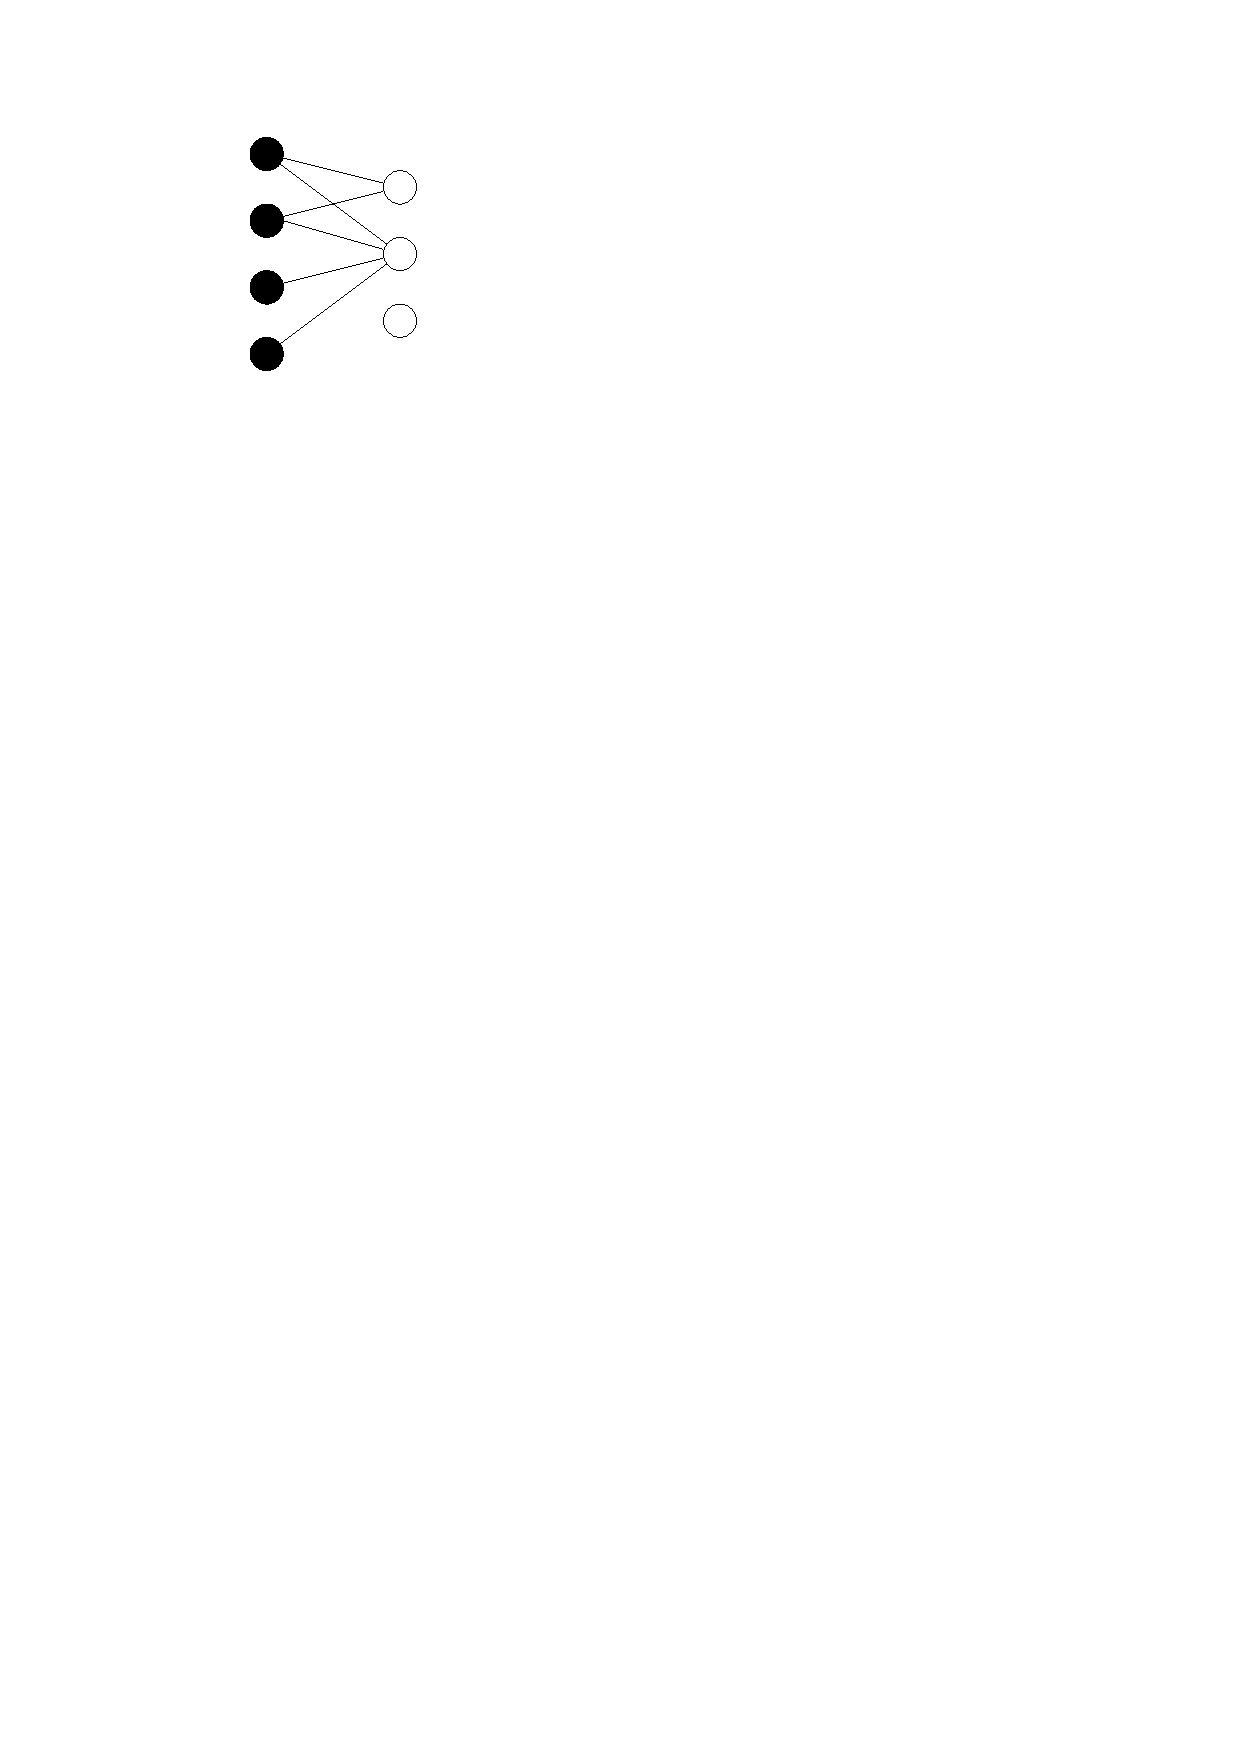
\includegraphics{bipartiteEx} 
\end{center}
\end{Boxample}

There are exponentially many partitions of $V$ into two subsets so we
do not want to have to test all possibilities to determine whether $V$ is bipartite.

\begin{Definition}
Let $k$ be a positive integer. A graph $G$ has a \defnfont{$k$-colouring}
if $V(G)$ can be partitioned into $k$ nonempty disjoint subsets such
that each edge of $G$ joins two vertices in different subsets.
\end{Definition}

\begin{Example}
The graph in \cref{ex:bipartite} has a 2-colouring as indicated.
\end{Example}

It is not just a coincidence that our example of a bipartite graph
has a 2-colouring.

\begin{Theorem} 
The following conditions on a graph $G$ are equivalent.
\begin{itemize}
  \item $G$ is bipartite.
  \item $G$ has a $2$-colouring.
  \item $G$ does not contain an odd length cycle.
\end{itemize}
\end{Theorem}
\begin{proof} 
Given a bipartition, use the same subsets to get a $2$-colouring, and
vice versa. This shows the equivalence of the first two conditions. Now
suppose $G$ is bipartite.  A cycle must have even length, since the start
and end vertices must have the same colour. Finally suppose that $G$
has no odd length cycle. A $2$-colouring is obtained as follows. Perform
BFS and assign each vertex at level $i$ the ``colour" $i \bmod 2$. If we
can complete this procedure, then by definition each vertex goes from
a vertex of one colour to one of another colour. The only problem could
be if we tried to assign a colour to a node $v$ that was adjacent to a
node $w$ of the same colour at the same level $k$. But then a cycle of
length $2k+1$ is created.
\end{proof}

It is now easy to see that we may use the method in the proof above
to detect an odd length cycle if it exists, and otherwise produce a
$2$-colouring of $G$. This of course runs in linear time.


%\section{Maximum matchings}
%\label{sec:matching}
%
%Next we want to introduce an important graph problem that can
%be solved in polynomial time by a clever path augmentation algorithm.  
%
%\begin{Definition}
%A \defnfont{matching} in a graph is a set of pairwise non-adjacent edges
%(that is, each vertex can be in at most one edge of the matching).
%A \defnfont{maximal matching} is a matching such that is not a proper subset
%of any other matching.
%A \defnfont{maximum matching} is one with the largest possible number of
%edges (over all possible matchings).
%\end{Definition}
%
%Often, for many real-world problems, we want to find a maximum matching 
%in bipartite graphs as illustrated by the next two examples.  
%
%\begin{Example}
%Suppose we have a set of workers $V_0$ and a set of tasks $V_1$ that need to be
%assigned.  A given worker of $V_0$ is able to perform a subset of the tasks in $V_1$.
%Now with each worker capable of doing at most one task at a time, the boss 
%would like to assign (match) as many workers as possible to as many of 
%the tasks. 
%\end{Example}
%
%\begin{Example}\label{ex:mp}
%Consider mating fussy kakapo who all live in differnt zoos.  We have a set of males  and females (as vertices) and edges 
%representing compatible mates.  The goal is to mate as many kakapo
%as possible in the current season, which is the same as finding a maximum matching in the
%relationship graph. This is traditionally called the \defnfont{marriage problem}
%\end{Example}
%
%In \cref{fig:matchbipartite} we illustrate the difference between
%a maximal and maximum matching in the setting of \cref{ex:mp}.
%The matchings consist of bold-dashed edges (between females on the left
%and males on the right) in the drawings.
%
%\begin{figure}
%\centering
%\includegraphics{bipartiteMatching}
%\caption{A maximal and maximum matching in a bipartite graph.}
%\label{fig:matchbipartite}
%\end{figure}
%
%It is easy to find a maximal matching $M$ in a graph. For example, 
%a simple greedy approach of
%iterating over all edges and adding each edge to $M$ if it is
%non-adjacent to anything already in $M$ will work.  As illustrated in
%\cref{fig:matchbipartite}, a maximal matching may have fewer
%edges than a more desirable maximum matching.
%
%Our algorithm to compute a maximum matching will be based on
%trying to improve an existing matching $M$ by finding certain
%types of paths in a graph.
%
%\begin{Definition}
%Given a matching $M$, an \defnfont{alternating path} is a path in which 
%the edges 
%of the path alternate from being in the matching and not.
%An \defnfont{augmenting path} is an alternating path that starts from and ends 
%on unmatched vertices.
%\end{Definition}
%
%For example, consider the augmenting path Eve--Doug--Cher--Fred of
%\cref{fig:matchbipartite}.  It contains three edges but only the
%middle edge is part of a matching on the left case.  We can get the
%better matching on the right if we add Eve-Doug, remove Doug--Cher, and add 
%Cher--Fred to the existing matching.  Thus, in general, we see that we can 
%improve a matching if we can find an augmenting path.  Note that there is always one
%more non-matching edge than matching edge in an augmenting path.
%Likewise, it is pretty easy to show that if there is no such augmenting path 
%then we must have a maximum matching (see Exercise~\ref{ex:agpath}).
%
%We next present a polynomal-time algorithm that finds an augmenting path if
%one exists.  The basic idea is to start from an unmatched vertex $v$
%and build a tree (via a graph traversal algorithm such as BFS) 
%of alternating paths away from $v$.  If we reach another unmatched vertex 
%then we have found an augmenting path.  Otherwise, if we visit all vertices
%(in the same component as $v$) then we conclude that no augmenting 
%path exists starting at $v$.  This algorithm is given in \cref{fig:augpath}.
%
%
%%\begin{algorithm}[H]
%%  \caption{An algorithm to find an augmenting path, given a matching
%%and an unmatched starting vertex.}
%%    \label{alg:augpath}
%%\begin{algorithmic}[1]
%%\Function{findAugmentingPath}{bipartite graph $G$; matching $M$; unmatched vertex $x$}
%%	\State queue $Q$
%%	\State array $\status[0..n-1]$, $\pred[0..n-1]$
%%	\For{$u \in V(G)$}
%%  		\State $\status[u] \gets $ WHITE; $\pred[u] \gets $ \texttt{null} 
%%	\EndFor
%%	\State $\status[x] \gets $ EVEN
%%	\State $Q$.\algfont{insert}$(x)$
%%	\While{\textbf{not}  $Q$.\algfont{isEmpty}$()$}
%%		\State $u \gets Q$.\algfont{pop}$()$
%% 		\If{$\status[u] =$ EVEN}
%% 			\For{each $v$ adjacent to $u$}
%% 				\If{$\status[v]$ = WHITE}
%% 					\State $\status[v] \gets$ ODD; $\pred[v] \gets$ u
%% 					\If{$v$ is unmatched in $M$}
%% 						\State \Return{path $x,\ldots, \pred[\pred[u]], \pred[u], u, v$}
%% 					\Else
%%	 					\State $Q$.\algfont{insert}$(v)$
%% 					\EndIf
%% 				\EndIf
%% 			\EndFor
%% 		\Else 			\Comment{that is, $\status[u] =$ ODD} 
%%			\State $v \gets$ matched vertex of $u$ from $M$
%%			\If{$status[v]$ = WHITE}
%%				\State$\status[v] \gets$ EVEN; $\pred[v] \gets u$
%% 				\State$Q$.insert$(v)$
%%	 		\EndIf
%% 		\EndIf
%%	\EndWhile
%%	\State \Return{false} \Comment{no augmenting paths containing $x$}
%%\EndFunction
%%\end{algorithmic}
%%\end{algorithm}
%
%
%
%\begin{Theorem}
%There exists a polynomial-time algorithm to find a maximum matching
%in a bipartite graph.
%\end{Theorem}
%%\begin{proof}
%%We first need to show that the algorithm \algfont{findAugmentingPath}, given in
%%\cref{fig:augpath}, does find an augmenting path if one exists.
%%It is sufficient to show that if there exists at least one augmenting path 
%%from vertex $x$ to some other unmatched vertex that we find any one of them 
%%(in our case, by imitating BFS, it will be one of shortest length).  
%%\algfont{findAugmentingPath}
%%builds a traversal tree starting at $x$ using the following constraints.
%%\begin{itemize}
%%\item If a reachable vertex $u$ is in the same partition as $x$ (status will
%%be set to EVEN by the algorithm) then we know (except for $x$) that there is 
%%an alternating path with the last edge including $u$ being in the matching.
%%\item If a reachable vertex $v$ is not in the same partition as $x$ (status will
%%be set to ODD if it is matched) then we know that there is 
%%an alternating path with the last edge including $v$ is not in the matching.
%%\end{itemize}
%%This process produces a tree with alternating paths rooted at $x$ as 
%%illustrated in \cref{fig:augtree}.  The status of the nodes are ODD 
%%or EVEN depending if they are an even or odd distance from $x$.  If a vertex 
%%(first seen) is at an odd distance then we have seen an alternating path 
%%where the last edge is not in the matching.  If this last vertex is unmatched 
%%then we have found an augmenting path, otherwise we extend the path by using 
%%the matched edge.  
%%If a vertex is at an even distance then we have seen an alternating path
%%where the last edge is in the matching.  Since the graph is bipartite the
%%status of being ODD or EVEN is unambiguous.
%%
%%\begin{figure}
%%\centering
%%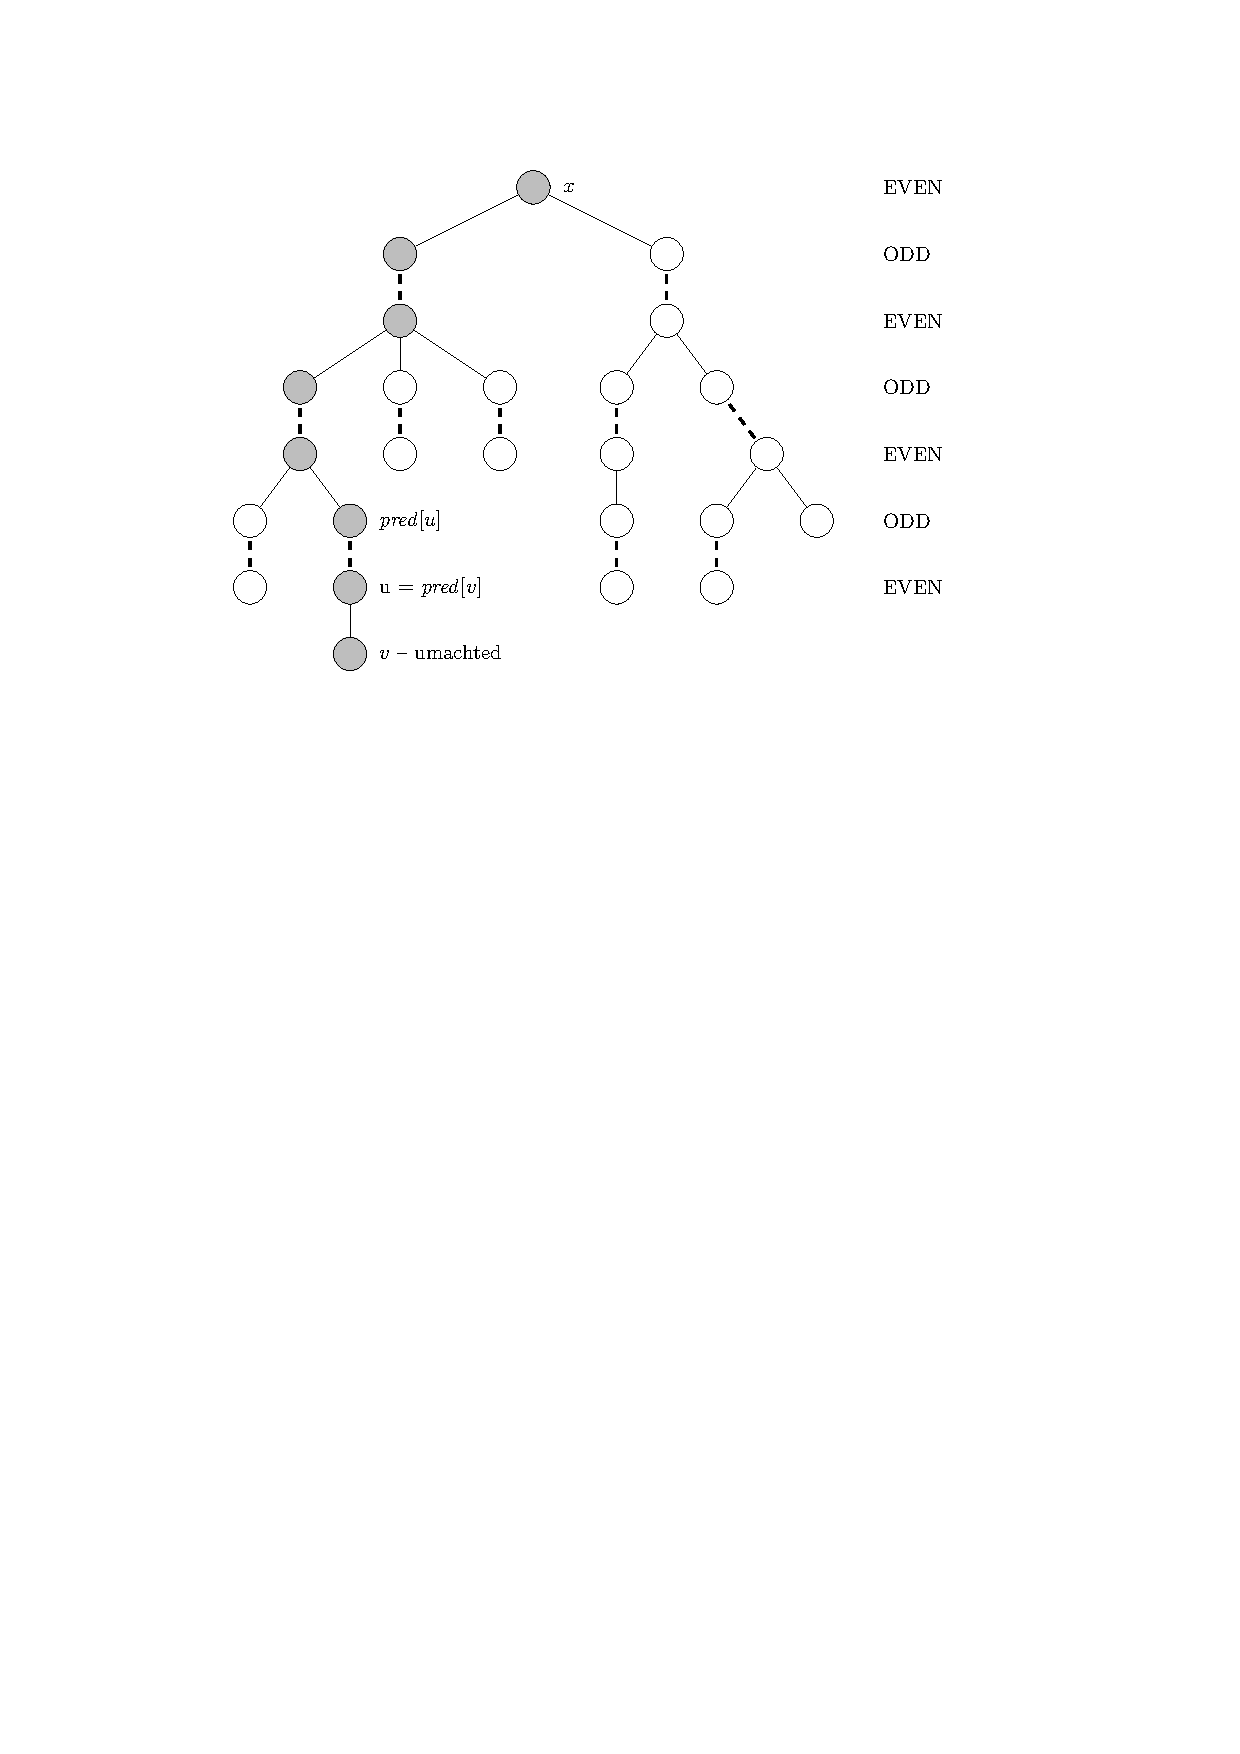
\includegraphics{augtree} 
%%\caption{Structure of the graph traversal tree for finding augmenting paths.}
%%\label{fig:augtree}
%%\end{figure}
%%
%%Suppose the algorithm \algfont{findAugmentingPath} terminates without
%%finding an augmenting path when one does exist.  Let $x=v_0,v_1,\ldots,v_k$
%%be a counterexample.  Consider the
%%first index $0<i\leq k$ such that $status[v_i] =$ WHITE.  We know $v_{i-1}$ was
%%inserted in the queue $Q$. Consider the two cases.  If $i-1$ is even then
%%since $v_i$ is a neighbour of $v_{i-1}$ its status would have changed to
%%ODD.
%%If $i-1$ is odd then either $(v_{i-1},v_i)$ is in the matching or not.
%%If so, the status of $v_i$ would have changed; if not, a prefix of the 
%%counterexample is not an augmenting path.  Thus, by contradiction,
%%\algfont{findAugmentingPath} will find an augmenting path if one exists.
%%
%%The running time of one invocation of \algfont{findAugmentingPath} is the same 
%%as the running time of BFS since each vertex is added to the queue $Q$
%%at most once.  For adjacency list representation of graphs this 
%%can be carried out in time $O(m)$.  If we find an augmenting path
%%then our best matching increases by one.  
%%Since a maximum matching is bounded by $\lfloor n/2 \rfloor$ we
%%only need to find at most $O(n)$ augmenting paths.
%%We potentially need to call \algfont{findAugmentingPath}
%%once for each unmatched vertex, which is bounded by $O(n)$, and 
%%repeat the process for each modified matching.  Therefore, the total 
%%running time to find a maximum matching is at most $O(n^2m)$.
%%\end{proof}
%
%The algorithm presented here can easily be improved to $O(nm)$ by
%noting that it is only required to traverse and compute an 
%``alternating path forest'' in order to find an augmenting path.  
%That is, we do not need to originate a call to \algfont{findAugmentingPath} for all 
%unmatched vertices. However the correctness is a bit tricky to justify.
%
%There are other algorithms that find maximum matchings more efficiently
%than the one presented.  One of these is the Hopcroft-Karp algorithm
%which runs in time $O(m\sqrt{n})$ and is based on finding a maximal 
%flow in a network (by adding a source and sink vertex and directing all edges
%from one vertex partition to the other of the bipartite graph).
%
%We conclude this section by mentioning that there also exist
%poly\-nomial-time algorithms to find maximum matchings in arbitrary
%(non-bipartite) graphs. The details are beyond the scope of this book.
%
%%\subsection*{Exercises}
%
%\begin{Exercise}\label{ex:agpath}
%Prove that a matching for a graph is maximum if and only if it does not
%have any augmenting paths.
%\end{Exercise}
%
%\begin{Exercise}
%Give an example of a bipartite graph of order 12 with a maximal matching 
%that has an augmenting path of length 5 and a maximum matching of 
%the same graph with two more edges.
%\end{Exercise}
%
%%\if 01
%%\begin{Exercise}
%%Explain what changes need to be done to the algorithm
%% \algfont{findAugmentingPath} 
%%so that it runs in time $O(|E|)$ and traverses all of the bipartite graph
%%(instead of just the tree reachable from the unmatched vertex $x$).
%%\end{Exercise}
%%\fi
%
%\begin{Exercise}\label{ex:konig}
%Show that the size of a maximum matching in a bipartite graph $G=(V,E)$ is the
%same as the size of the smallest \defnfont{vertex cover} of $G$.  A vertex cover
%is a subset $V' \subseteq V$ of vertices such that for 
%all $(u,v) \in E$, at least one of $u$ or $v$ is in $V'$.
%Does the equality hold for arbitrary graphs?
%\end{Exercise}
%
%\section{Notes}
%
%The linear-time algorithm for finding strong components of a digraph was 
%introduced by R. E. Tarjan in 1971.
%
%One of the early polynomial-time algorithms for finding
%maximum matchings in bipartite graphs is based on the Ford--Fulkerson 
%network flow algorithm \cite{FF56} from 1956.
%The first polynomial-time algorithm for finding a maximum matching in an 
%arbitrary graph was presented by J.~Edmonds \cite{Ed65} in 1965.

%[FF56]
%L. R. Ford and D. R. Fulkerson 
%"Maximal flow through a network". 
%\textit{Canadian Journal of Mathematics} \textbf{8} (1956), pp 399--404.

%[Ed65]
%J. Edmonds.  Paths, trees, and flowers
%\textit{Canadian Journal of Mathematics} \textbf{17} (1965), pp. 449-467. 
